%%%%%%%%%%%%%%%%%%%%%%%%%%%%%%%%%%%%%%%%
% datoteka diploma.tex
%
% vzorčna datoteka za pisanje diplomskega dela v formatu LaTeX
% na UL Fakulteti za matematiko in fiziko
%
% vkup spravil Gašper Fijavž, december 2010 množica popravkov v januarju,
% februarju marcu 2011 verzijo 29. marec 2011 za FMF 19.9.2013 prilagodil Rok
% Mihevc
%%%%%%%%%%%%%%%%%%%%%%%%%%%%%%%%%%%%%%%%

\documentclass[a4paper, twoside, 12pt]{book}

\usepackage[utf8]{inputenc}
\usepackage[slovene,english]{babel}    % naloži, med drugim,
\usepackage[pdftex]{graphicx}  % omogoča vlaganje slik
\usepackage{fancyhdr}          % poskrbi, na primer, za
\usepackage{amssymb}           % dodatni simboli
\usepackage{amsmath}           % eqref, npr.
\usepackage{verbatim}
% \usepackage{float}


%oznake strani
\renewcommand{\chaptermark}[1]

\newcommand{\BibTeX}{{\sc Bib}\TeX}
\newcommand{\autfont}{\Large}
\newcommand{\titfont}{\LARGE\bf}
\newcommand{\clearemptydoublepage}{\newpage{\pagestyle{empty}\cleardoublepage}}
\setcounter{tocdepth}{2}

\begin{document}

\selectlanguage{slovene}
\frontmatter
\setcounter{page}{1}
\renewcommand{\thepage}{}

\begin{center}
  {\large\sc Univerza v Ljubljani\\
    Fakulteta za Matematiko in Fiziko\\
    Oddelek za Fiziko\\
  Univerzitetni študij, naravoslovna smer}
  \vskip 10em
  {\autfont Rok Mihevc \par}
  {\titfont Kraške vrtače Dinarskega krasa \par}
  {\vskip 2em \textsc{DIPLOMSKO DELO}\par}
  \vfill
  \null
  {\large \textsc{Mentor}: prof.\ dr.  Rudolf Podgornik\par}
    %  {\large \textsc{Somentor}:  izr.\ prof.\ dr. \par}%
  {\vskip 2em \large Ljubljana, 2014 \par}
\end{center}

\def\thepage{}% preprecimo tezave s stevilkami strani v kazalu
\tableofcontents{}

\newpage \thispagestyle{empty}

\addcontentsline{toc}{chapter}{Povzetek} 
\chapter*{Povzetek}

  Z numeričnimi metodami obdelamo $60 km^2$ velik digitalni model reliefa Menišije ločljivosti $1m^2$ in identificiramo veliko število kraških vrtač. Iz oblik velikega števila vrtač izračunamo povprečno obliko vrtače in jo analitično opišemo z Gaussovo funkcijo. Odkrite realne vrtače nato prilegamo na Gaussovo funkcijo ter pogledamo porazdelitev parametrov le-te na našem vzorcu.

  Zaradi geološke zgodovine področja Menišije in medsebojne podobnosti vrtač na tem območju postavimo tezo, da jih je oblikoval isti geomorfološki proces, ki vodi do vsem skupne stabilne oblike, ki so jo vrtače na tem območju že dosegle.
  S pomočjo podatkov, pridobljenih v prvem delu naloge, predlagamo statičen nastavek, ki analitično opiše najdene vrtače. Postavimo tezo, da vrtače oblikuje stohastična denudacija površja, ter primerjamo teoretično pričakovan eksponent hrapavosti z izmerjenim. Pogledamo še nekaj determinističnih difuzijsko-reakcijskih sistemov, ki bi lahko služili kot dinamični model nastanka vrtač.

\vspace*{1cm}

\noindent \textbf{Ključne besede:} Digitalni model reliefa, obdelava slik, vrtača, kras, razvoj reliefa, stohastične diferencialne enačbe, dinamične enačbe
\smallskip

\noindent \textbf{PACS:} 95.75.Mn, 02.50.Ey 02.60.Cb, 02.60.Ed, 68.35.Ct, 68.35.Fx

\newpage \thispagestyle{empty}

\selectlanguage{english} \addcontentsline{toc}{chapter}{Abstract}
\chapter*{Abstract}

  Using numerical methods we analyzed $60 km^2$ of $1m^2$ resolution digital terrain model of Menišija and identified a large number of karst Dolines. We calculated average shape of a large number of Dolines and analytically described it by a Gaussian function. We then fitted the real Dolines to a Gaussian function and studied the distribution of parameters in our sample from Menišija.

  Due to the geological history of Menišija and similarity of Dolines in the area we propose that they were shaped by the same geomorphological process, that ultimately leads to a common stable form that was already reached by the sinkholes in this area.
  Using the data acquired in the second chapter we propose a static Ansatz that describes found Dolines. We propose a thesis that Dolines are formed by stochastic surface denudation, and compare the theoretically derived roughness exponent with the one measured on relief data from Menišija. Then we study several diffusion-reaction systems, which could serve as dynamic models of Dolines.

\vspace*{1cm}

\noindent \textbf{Keywords:} Digital relief model, image processing, dolines, karst relief evolution, stochastic differential equations, dynamic equations
\smallskip

\noindent \textbf{PACS:} 95.75.Mn, 02.50.Ey 02.60.Cb, 02.60.Ed, 68.35.Ct, 68.35.Fx

\selectlanguage{slovene}

\newpage \thispagestyle{empty}

\mainmatter
\setcounter{page}{1}
\pagestyle{fancy}
\rhead{\thepage}


  \chapter{Uvod}
  \label{ch:uvod}



  Namen tega dela je na podlagi digitalnega modela reliefa dokumentirati in statistično preučiti velik vzorec kraških vrtač na slovenskem Dinarskem krasu, predlagati analitično funkcijo, ki bi opisala idealno vrtačo, ter na podlagi le-te poskusiti modelirati dejavnike, ki povzročajo nastanek in obliko vrtač.

Vrtače so zaobljene lijakaste globeli, globine nekaj metrov in premera nekaj deset metrov. Najdemo jih na starih kraških poljih in planotah po celotnem Dinarskem krasu. Primer starega polja z razvitimi vrtačami: (Slika \ref{fig:vrtace-bpetrovac}). 

  \begin{figure}[h]
    \begin{center}
      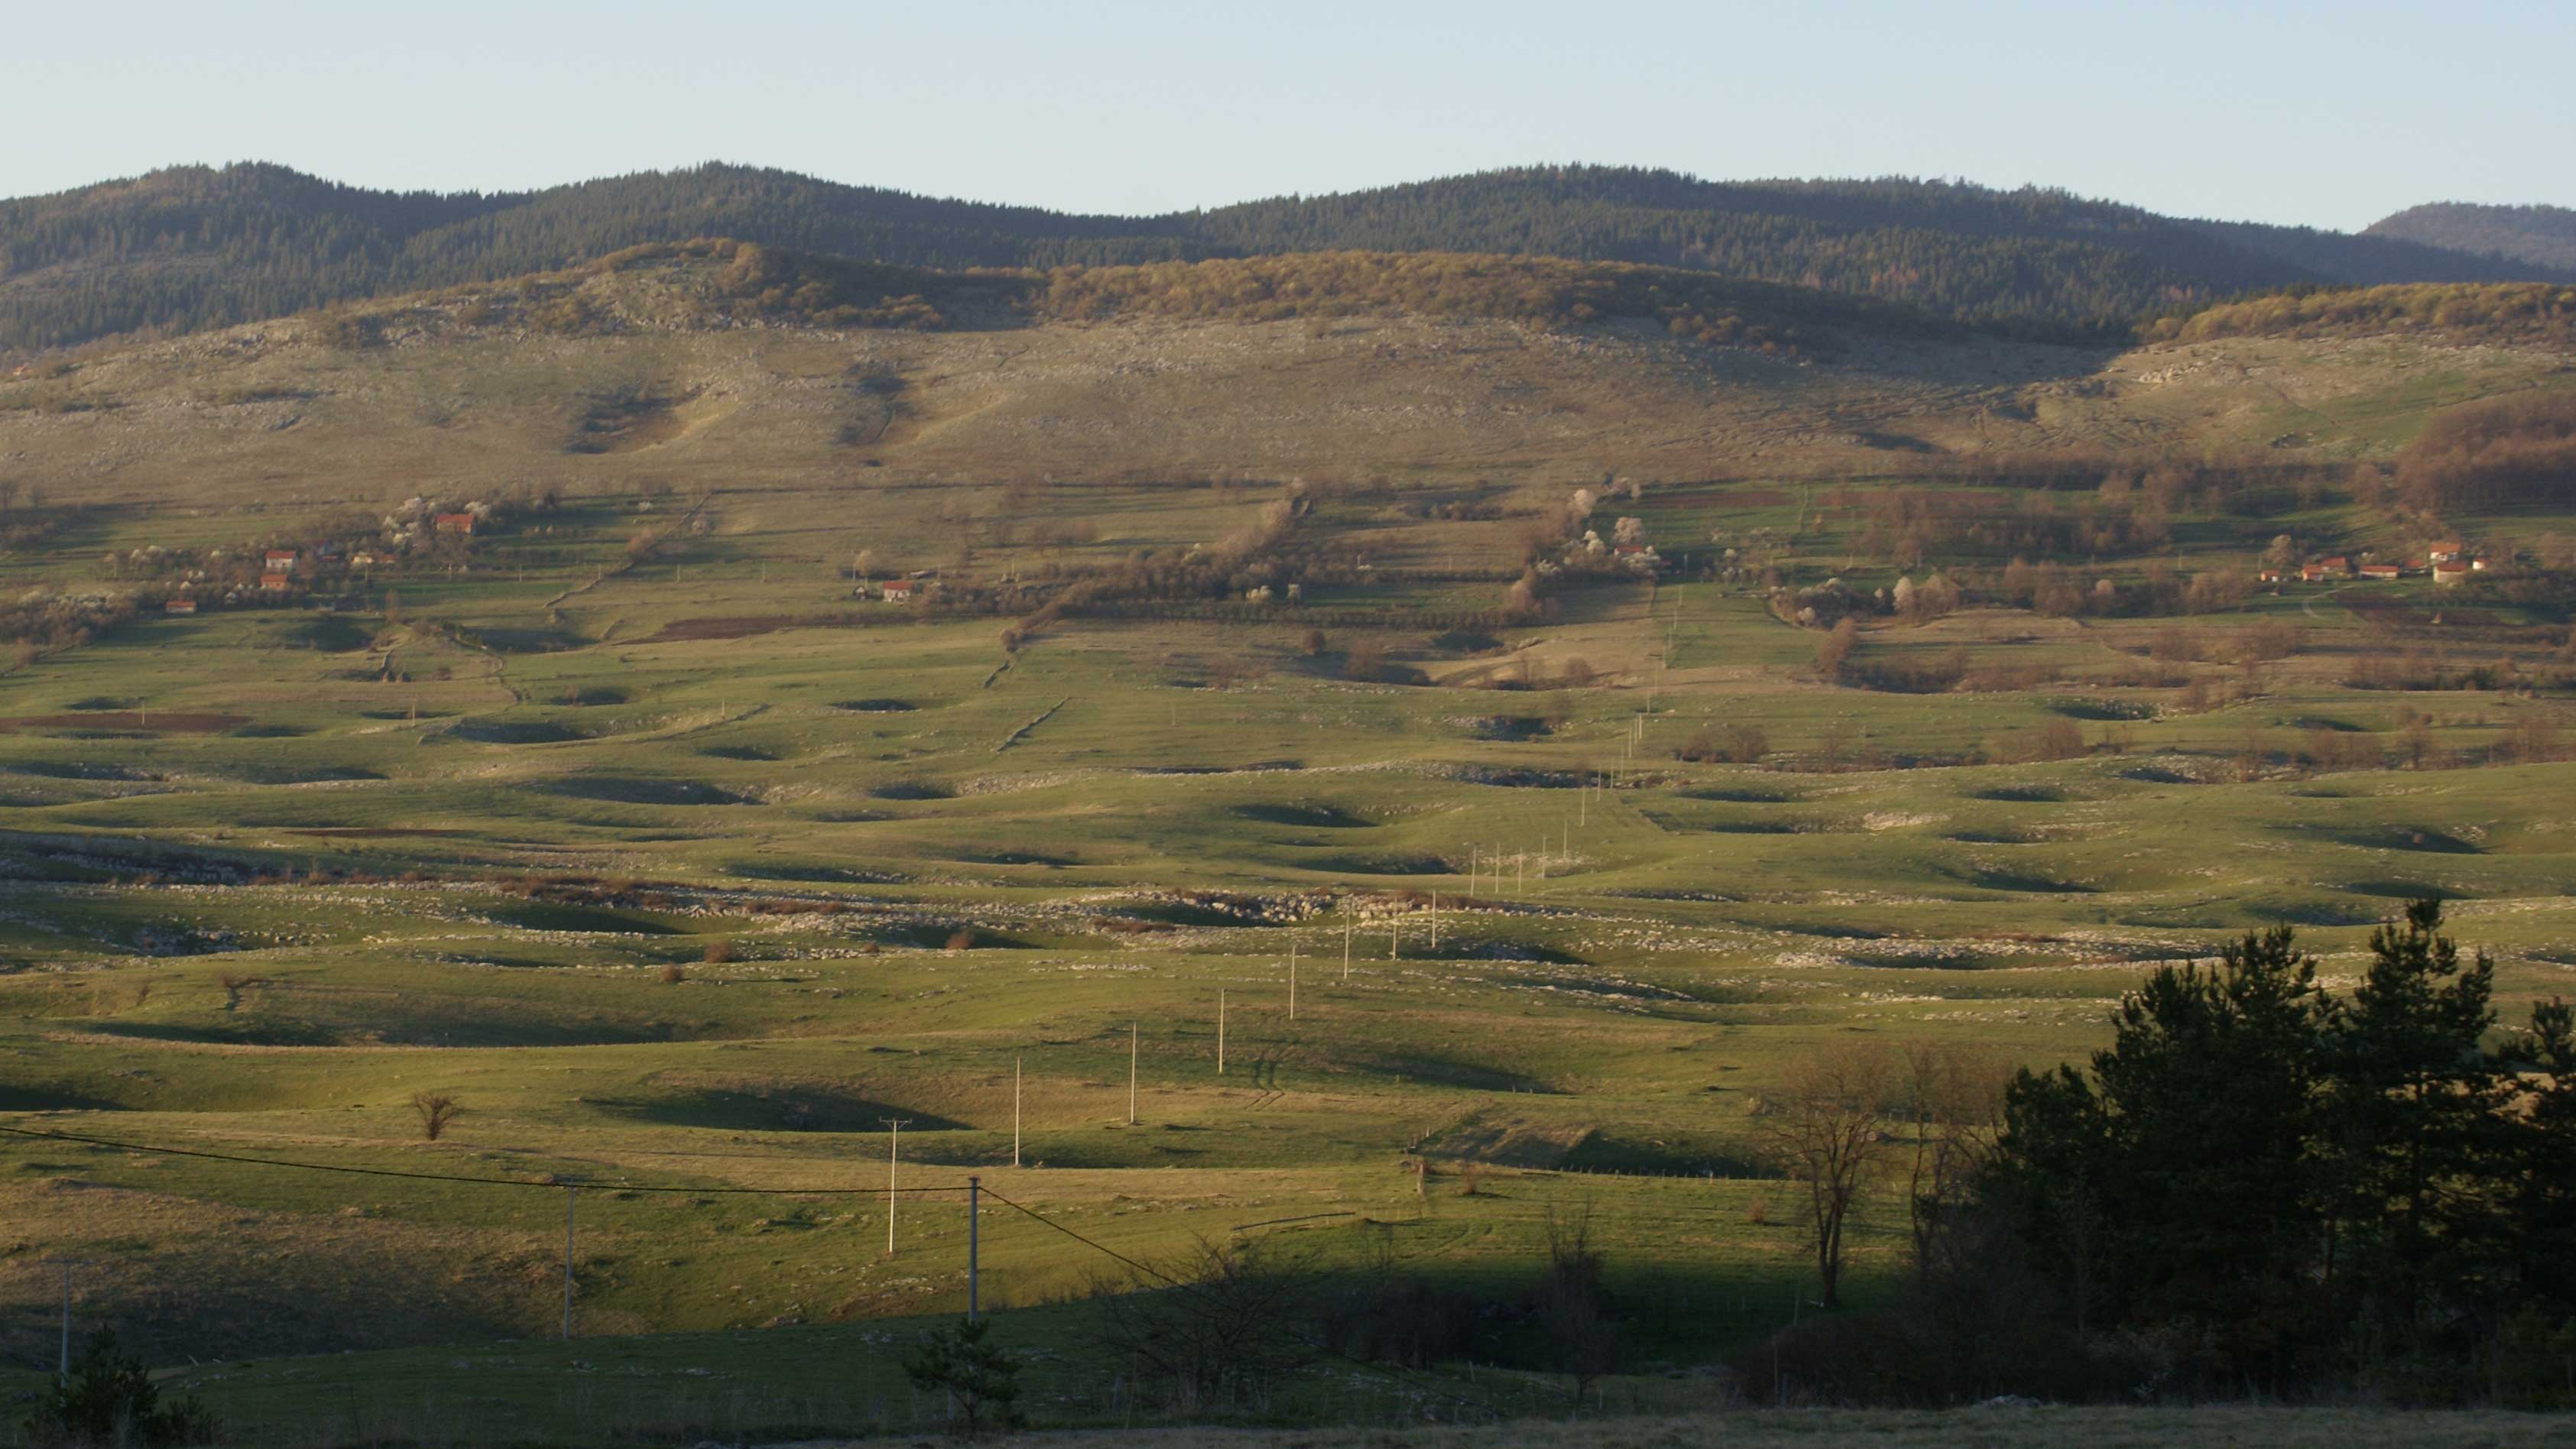
\includegraphics[width=10cm]{slike/bpetrovac}
    \end{center}
    \caption{Skupina vrtač vrezanih v staro kraško polje v bližini Bosanskega Petrovca, BiH \cite{bpetrovac}.}
    \label{fig:vrtace-bpetrovac}
  \end{figure}

Najširše sprejet model nastanka vrtač v geomorfološki literaturi podata Ford in Williams \cite{ford2007karst}: (Slika \ref{fig:vrtaca-ford-williams}). Na ta model se bomo oprli, ko bomo poskusili modelirati dinamiko vrtač.

  Za študij realnih vrtač uporabimo digitalni model reliefa Menišije (Slika \ref{fig:menisija-karta}) ločljivosti 1m, ki nam da natančno višinsko karto velike količine vrtač, ter omogoči zanesljivo identifikacijo in študij tega pojava (Slika \ref{fig:menisija-relief}).

  \begin{figure}[h]
    \begin{center}
      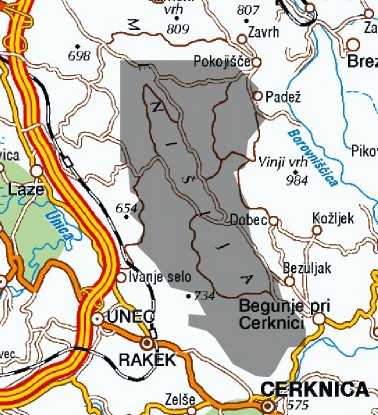
\includegraphics[width=6cm]{slike/menisija-karta}
    \end{center}
    \caption{Menišija, $60 km^2$ veliko območje med Cerknico in Logatcem, vsebuje nekaj tisoč vrtač ter nekaj udornic in predstavlja približno odstotek slovenskega krasa. Osenčen del zemljevida označuje področje digitalnega modela reliefa uporabljenega v tej nalogi (Slika \ref{fig:menisija-relief}). Vira: Geopedia, Geodetski inštitut Slovenije.}
    \label{fig:menisija-karta}
  \end{figure}

  Površje Menišije sestavljajo plasti krednega apnenca (starost nastanka 135-65 milijonov let), ki so bili zaradi dogodkov, povezanih s podrivanjem Adriatske plošče v Miocenu (17-7 milijonov let) prišli na površje. Območje Menišije je bilo do 3.5 milijona let pred sedanjostjo s poplavami uravnavano kraško polje, nato pa se je zaradi tektonske aktivnosti dvignilo nad okolico. S tem se je uravnavanje prenehalo in vzpostavljeni so bili geomorfološki pogoji za nastanek vrtač.
Hitrost zniževanja (denudacije) kraškega površja zaradi kemičnega preperevanja apnenca, se ocenjuje na 20-50 m / milijon let, torej se je površje Menišije v času od prenehanja uravnavanja znižalo za 70-175m, hkrati pa so se v njem pojavile vrtače, udornice in brezstrope jame. \cite{Vrabec2006} \cite{Placer2010}

Denudacijo kraškega površja povzroča kemična erozija apnenca. Apnenec raztaplja šibka ogljikova kislina, ki nastane z raztapljanjem ogljikovega dioksida v vodi. Na mestih, kjer se voda ne more zadrževati, na primer na goli skali, je denudacija počasnejša, oblikujejo se škraplje in žlebiči velikosti od nekaj milimetrov do nekaj metrov. Kraška polja, velikosti od deset do sto km, ki so pogosto poplavljena, pa denudacija uravna.

Iz geologije torej izvemo, da se je uravnano površje Menišije v obdobju 3.5 milijonih let zaradi raztapljanja kamnine stalno zniževalo, hkrati pa se je na njem pojavilo veliko število vrtač. Vrtače take velikosti in oblike najdemo tudi v drugih delih Dinarskega krasa, na področjih kjer so bili pogoji za nastanek vrtač vzpostavljeni prej ali kasneje kot v Menišiji.

Iz tega sklepamo, da se bodo pri določenih pogojih na ravnem kraškem površju sčasoma oblikovale vrtače. Če so vrtače, po dolgem času, podobnih si dimenzij, sklepamo da konvergirajo proti stabilni obliki, ki je po dolgem času odvisna le od lokalnih pogojev.

Da dinamiko vrtač bolje osvetlimo, bomo v (Poglavje \ref{realne-vrtace}) pregledali velik vzorec vrtač, ki nam ga nudi LiDARski posnetek Menišije in poročali kakšne vrtače tam najdemo. Nato bomo v (Poglavje \ref{analiticno-modeliranje}) dobljeni povprečni vrtači poskusili z različnimi prijemi pripisati časovno dinamiko.
 

  \chapter{Realne vrtače}
  \label{realne-vrtace}

V tem poglavju bomo iz celotnega LiDARskega posnetka Menišije (Slika \ref{fig:menisija-relief}) izbrali kraške vrtače in predlagali funkcijo, ki jih v povprečju opiše. Nato bomo to funkcijo prilegali na posamezne vrtače in komentirali porazdelitev parametrov funkcije.

  \section{Segmentacija vrtač}

Identifikacijo velike količine objektov se lotimo s segmentacijo po indeksu konkavnosti, kot predlaga \cite{doctor13} - uvedemo lokalni indeks konkavnosti $I_k$ (\ref{ik}), ki ga izračunamo tako, da od izbrane točke v matriki višinskih točk odštejemo povprečno vrednost točk, izbrani točki koncentričnega kolobarja:
\begin{equation}  I_k(r_0,r_1,r_2) = h(r_0)- \frac{1}{N}\sum\limits_{r_1<r<r_2} h(r). \label{ik} \end{equation}

  \begin{figure}[h!]
    \begin{center}
      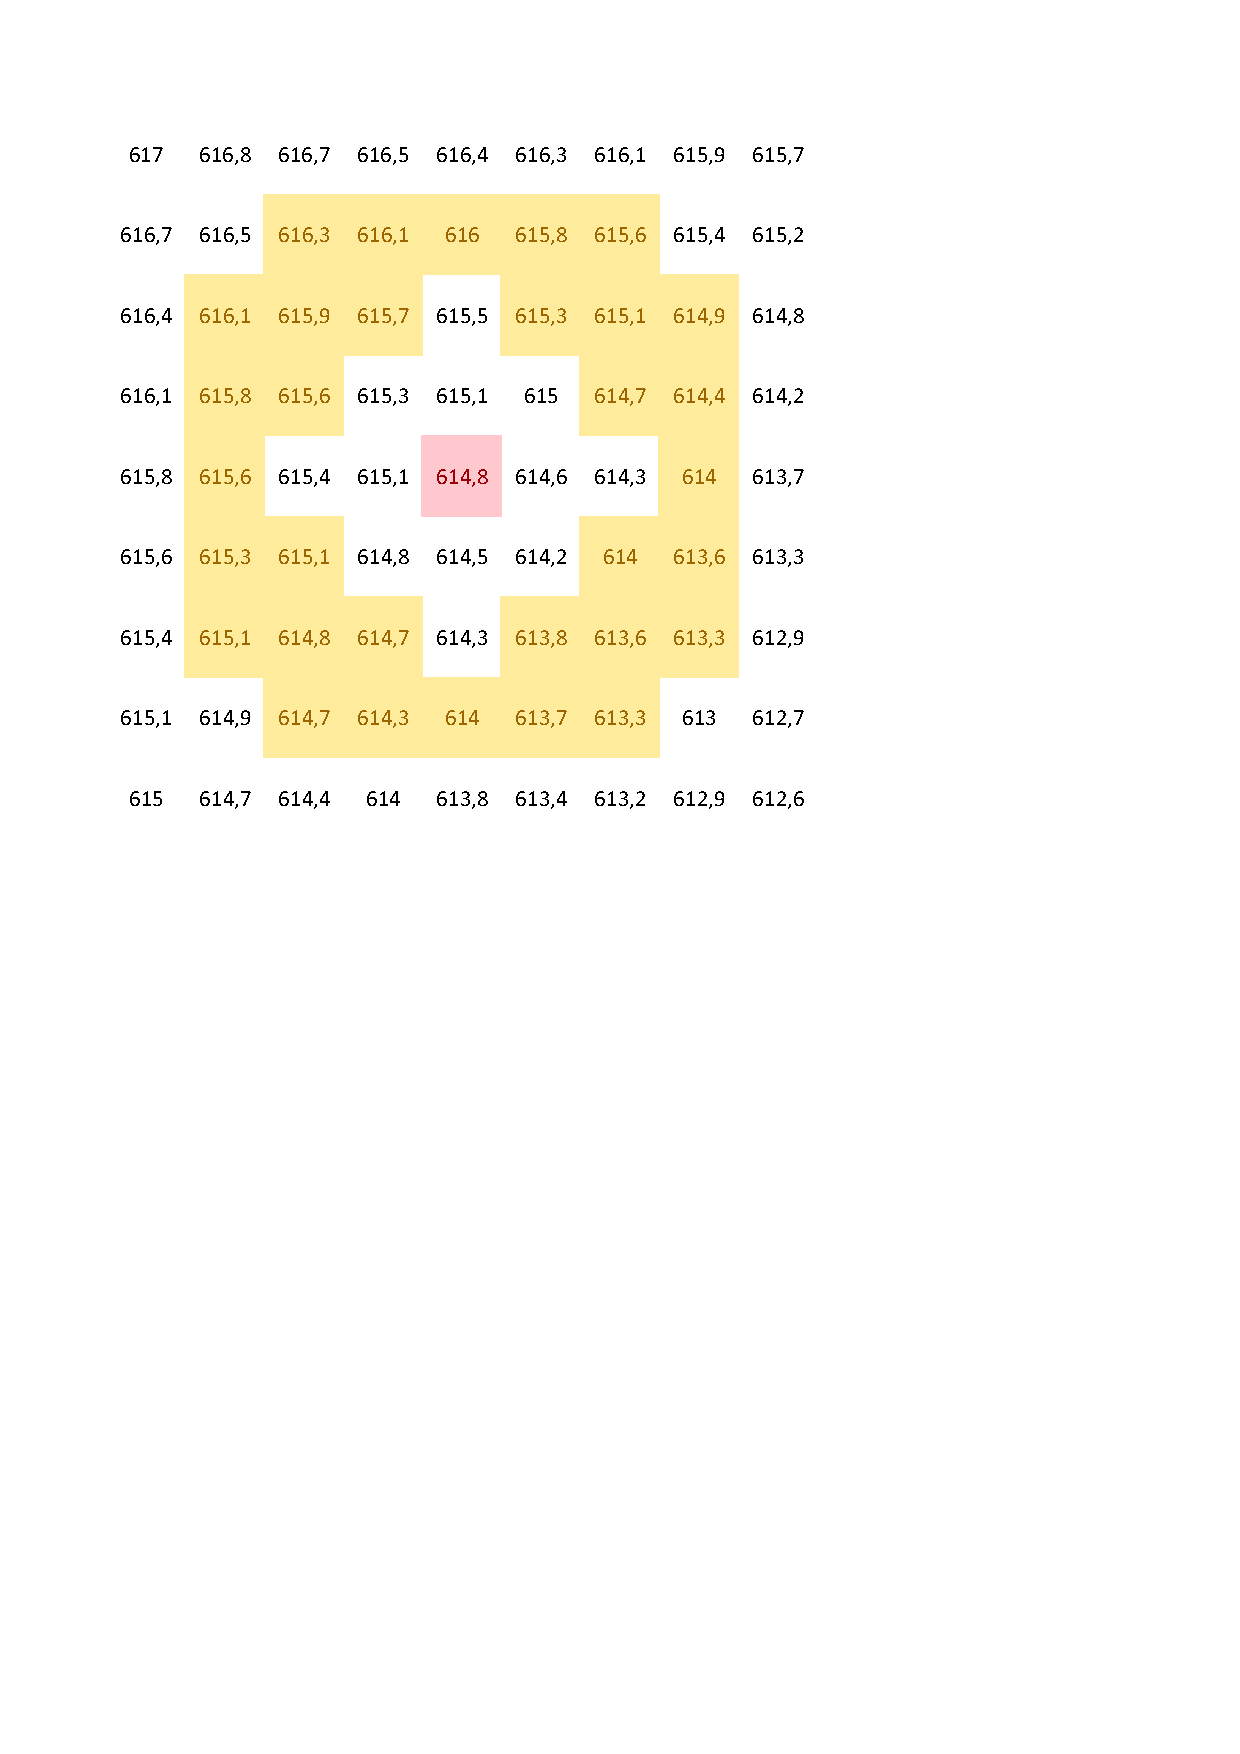
\includegraphics[width=4cm]{slike/concavity-ring-visualisation-2}
    \end{center}
    \caption{V prikazanem primeru je indeks konkavnosti, $I_k = 614,8 - 19676,2/32 = - 8,125 \cdot 10^{-2}$.}
    \label{fig:concavity-ring}
  \end{figure}

Center kolobarja postavimo v točko katere indeks konkavnosti računamo, $r_1$ in $r_2$ pa sta notranji ter zunanji radij kolobarja.
Primer kolobarja vidimo na (Slika \ref{fig:concavity-ring}). Indeks konkavnosti izračunan na konkavni ploskvi bo negativen, na konveksni pa pozitiven. Če ima ploskev konkavna in konveksna področja, bo rezultat odvisen tudi od izbire okolice.

Postopek ponovimo po celotni matriki višinskih točk. Rezultat je matrika indeksa konkavnosti.

Od dimenzij, ki jih izberemo za kolobar je odvisno, ali bodo določene točke v reliefu imele pozitven ali negativen indeks konkavnosti. Empirično se odločimo za tri kolobarje različnih velikosti $(r_1=10,r_2=15;r_1=15,r_2=25;r_1=60,r_2=100)$, za katere ocenimo da z njimi najdemo največ vrtač. Z njimi izračunamo indeks konkavnosti, ki je prikazan na (Slika \ref{fig:concavity-samples}).

  \begin{figure}[h!]
    \begin{center}
      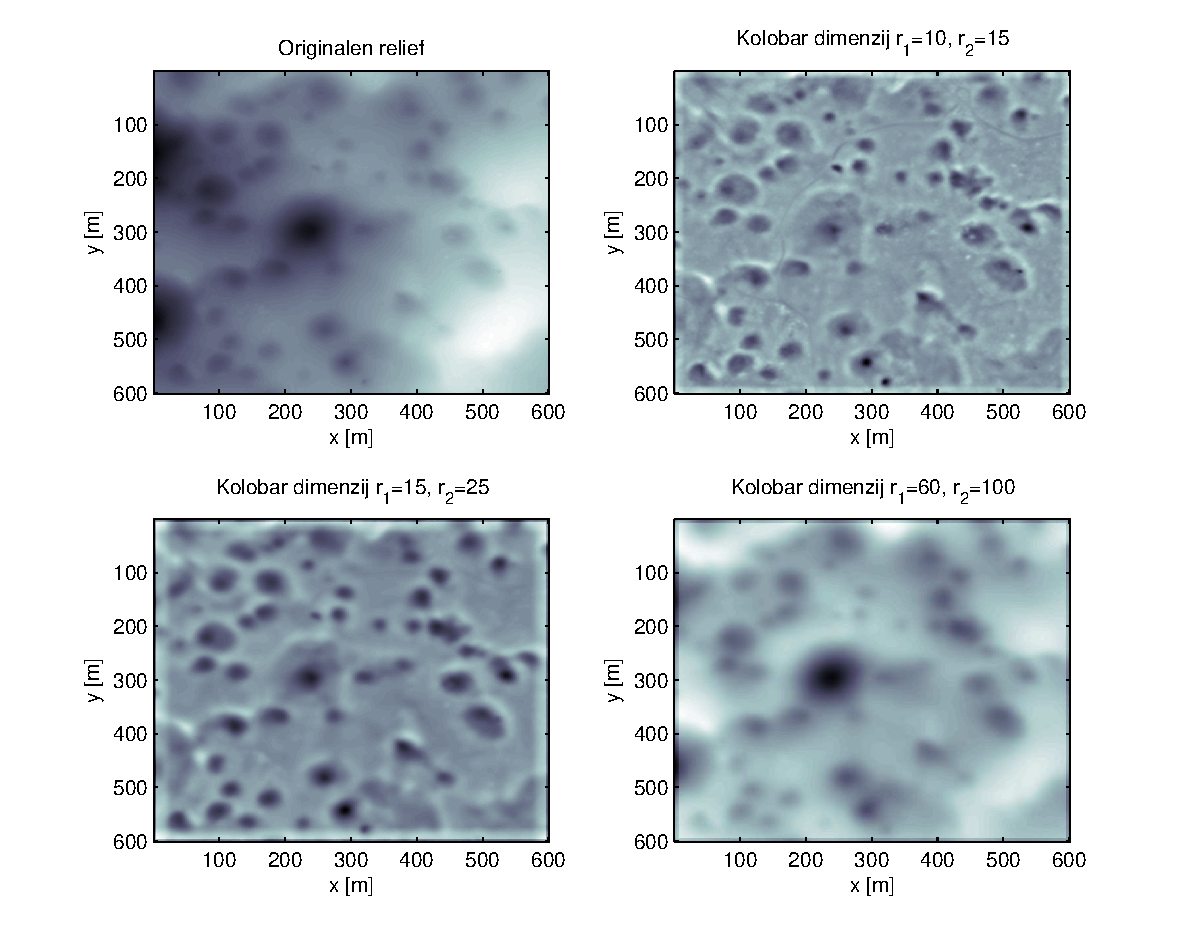
\includegraphics[width=12cm]{slike/concavity-samples}
    \end{center}
    \caption{Indeks konkavnosti reliefa $I_k$ definiranega v (\ref{ik}), pri različno izbranih dimenzijah kolobarja $(r_1=10,r_2=15;r_1=15,r_2=25;r_1=60,r_2=100)$.}
    \label{fig:concavity-samples}
  \end{figure}

Izračunamo standardni odklon indeksa konkavnosti $\sigma_{I_k}$. Arbitrarno odločimo, da so konveksni tisti deli površja (svetlejši odtenki), kjer je $I_k > -\frac{\sigma_{I_k}}{2}$. Zavržemo jih in konkavne (temnejši odtenki) dele površja odberemo kot vrtače. Vidimo, da pri izbiri manjšega kolobarja najdemo več vrtač, a podcenimo njihovo velikost. Pri izbiri večjega kolobarja pa se zgodi, da več manjših vrtač prepoznamo kot eno veliko. Zato vse tri rezultate primerjamo in v primeru, da večja vrtača prekriva eno manjšo, izberemo večjo vrtačo in zavržemo manjšo. V primeru da velika vrtača prekrije več manjših izberemo manjše. Rezultat je segmentacija vrtač na (Slika \ref{fig:concavity-segmentation-samples}).
  \begin{figure}[h!]
    \begin{center}
      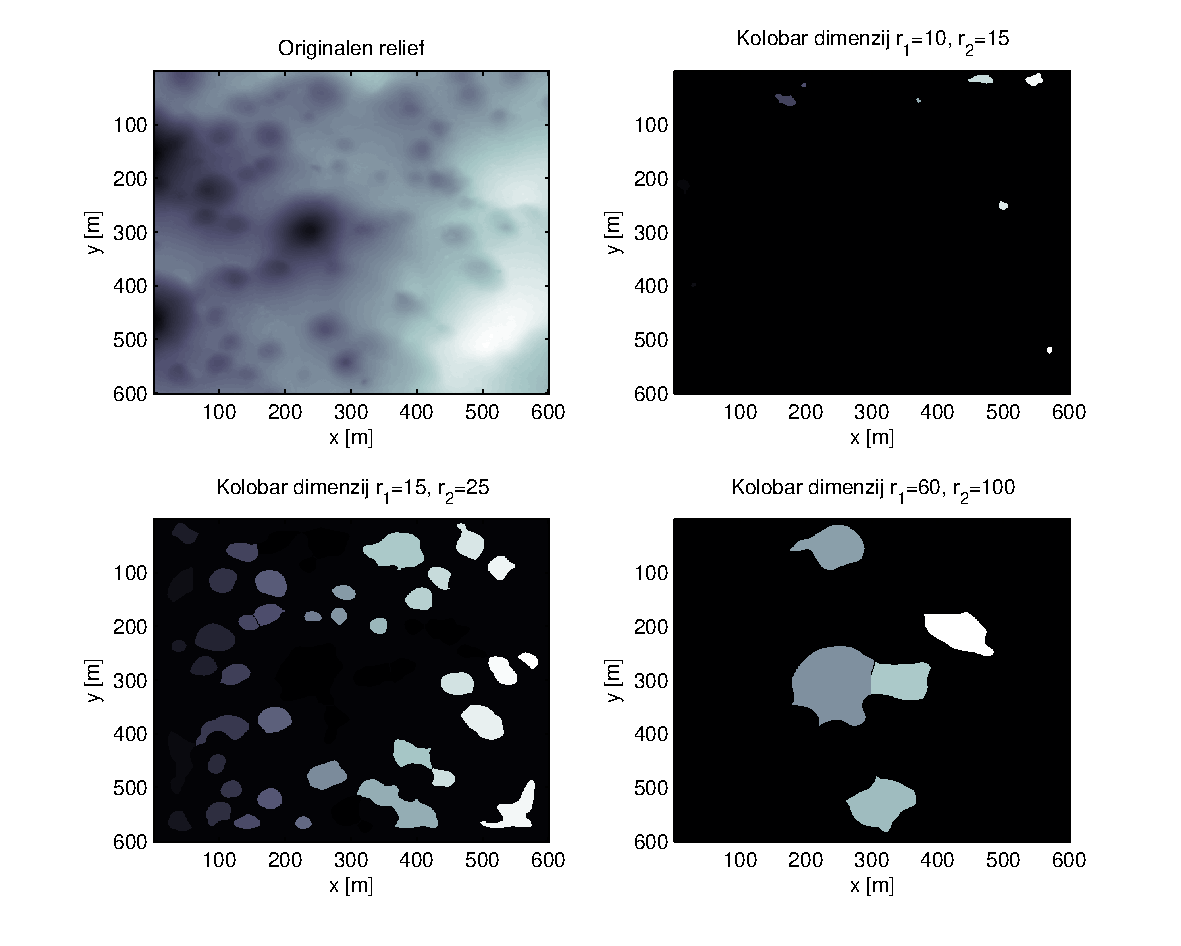
\includegraphics[width=12cm]{slike/concavity-segmentation-samples.pdf}
    \end{center}
    \caption{Indeks konkavnosti reliefa $I_k$ definiranega v (\ref{ik}), pri različno izbranih dimenzijah kolobarja $(r_1=10,r_2=15;r_1=15,r_2=25;r_1=60,r_2=100)$.}
    \label{fig:concavity-segmentation-samples}
  \end{figure}
Sedaj vrtače zarišemo preko večjega senčenega reliefa: (Slika \ref{fig:menisija-vrtace}). Opazimo, da kljub trudu nekoliko podcenimo velikost vrtač. Za statistično analizo to ni moteče, saj podcenitev napravimo na vseh vrtačah in na enak način.
  \begin{figure}[h]
    \begin{center}
      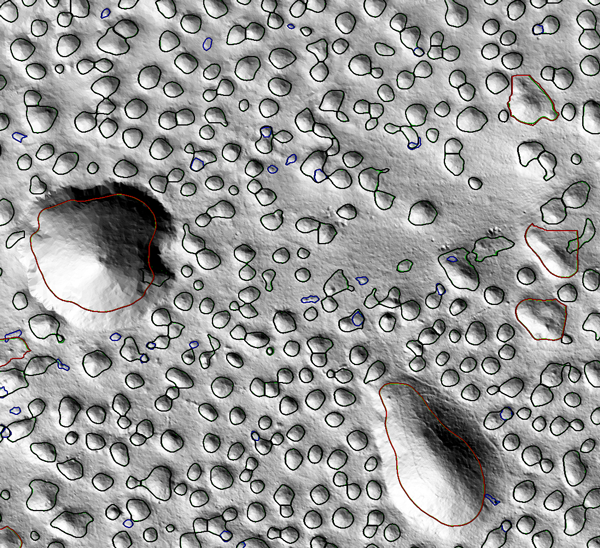
\includegraphics[width=7cm]{slike/menisija-vrtace}
    \end{center}
    \caption{Del od 8687 zaznanih vrtač na območju Menišije. Poleg vrtač so na sliki vidni tudi dve udornici. Vrtače, ki smo jih zaznali pri izbiri manjšega kolobarja so obkrožene z modro barvo, vrtače srednjega kolobarja z črno in vrtače velikega z rdečo. Pri udornicah je posebno opazna podcenitev velikosti.}
    \label{fig:menisija-vrtace}
  \end{figure}

  \section{Analiza}

  Površino vrtač definiramo s številom višinskih točk (pikslov), ki jo sestavljajo:
    \begin{equation}
      A = \sum pikslov.
    \end{equation}

S to količino nato predpostavimo efektivni polmer objektov:

    \begin{equation} 
      r_{eff} = \sqrt{\frac{A}{\pi}}. 
    \end{equation}

Porazdelitev efektivnih polmerov pokažemo na histogramu (Slika \ref{fig:menisija-polmeri-hist}).
  \begin{figure}[h!]
    \begin{center}
      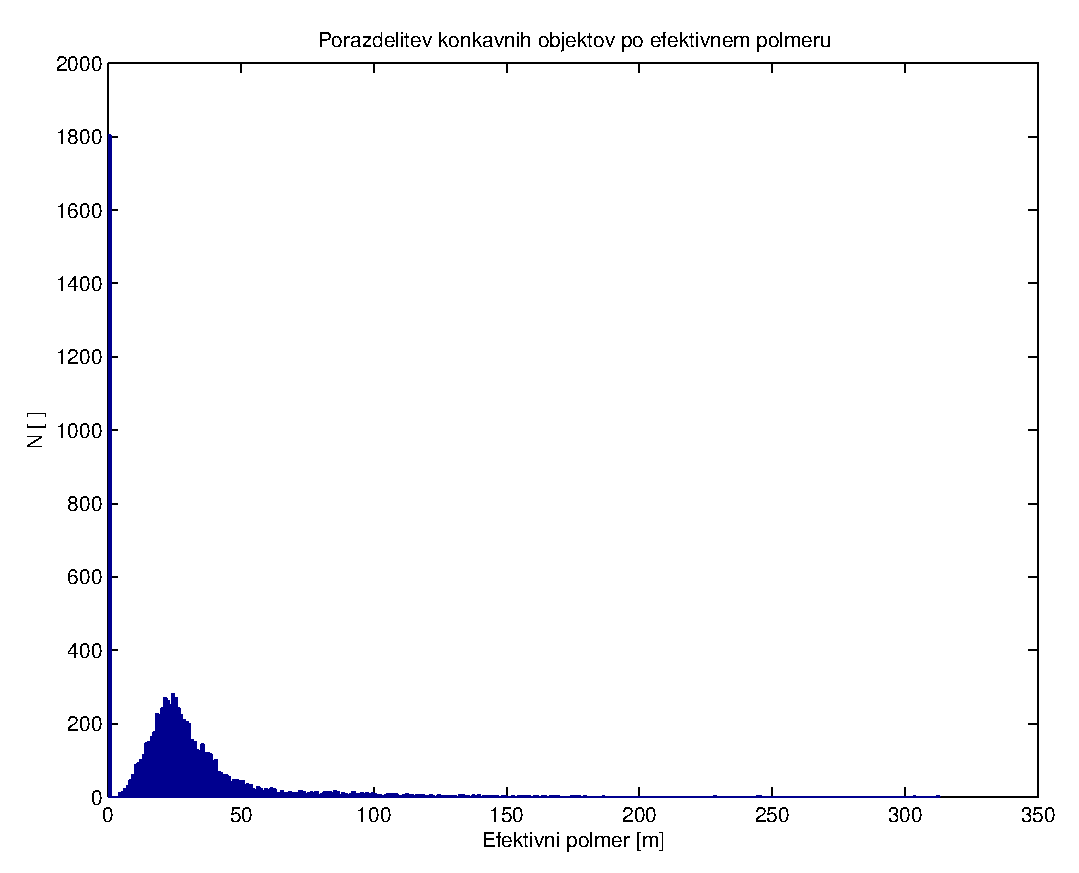
\includegraphics[width=14cm]{slike/menisija-polmeri-hist}
    \end{center}
    \caption{Polmeri konkavnih objektov v Menišiji. Povprečen efektivni polmer objekta je $\bar r_{eff}=26m$, standardna deviacija efektivnega polmera pa je $\sigma_{r_{eff}}=24m$.}
    \label{fig:menisija-polmeri-hist}
  \end{figure}
Povprečen efektivni polmer objekta je $\bar r_{eff}=26m$, standardna deviacija efektivnega polmera pa $\sigma_{r_{eff}}=24m$. Za $71\%$ objektov še velja: $2m < r_{eff} < 50m$.
S smiselno velikostjo objektov in pregledom vizualizirane segmentacije (Slika \ref{fig:menisija-vrtace}) preverimo, da so najdeni objekti res vrtače.

  Posamezne realne vrtače zaradi lokalnih pogojev in zgodovine razvoja reliefa niso simetrične, a zdi se, da so si med seboj podobne. Da bi ugotovili statistično najverjetnejšo obliko vrtače, izračunamo povprečje velikega števila realnih vrtač. Uporabimo dva pristopa - pri prvem (Slika \ref{fig:menisija-vrtaca}) vrtače različnih velikosti raztegnemo na isto velikost in povprečimo, pri drugem (Slika \ref{fig:menisija-vrtace-po-razredih}) pa jih razdelimo v velikostne razrede in jih povprečimo znotraj le-teh.

  \begin{figure}[h!]
    \begin{center}
      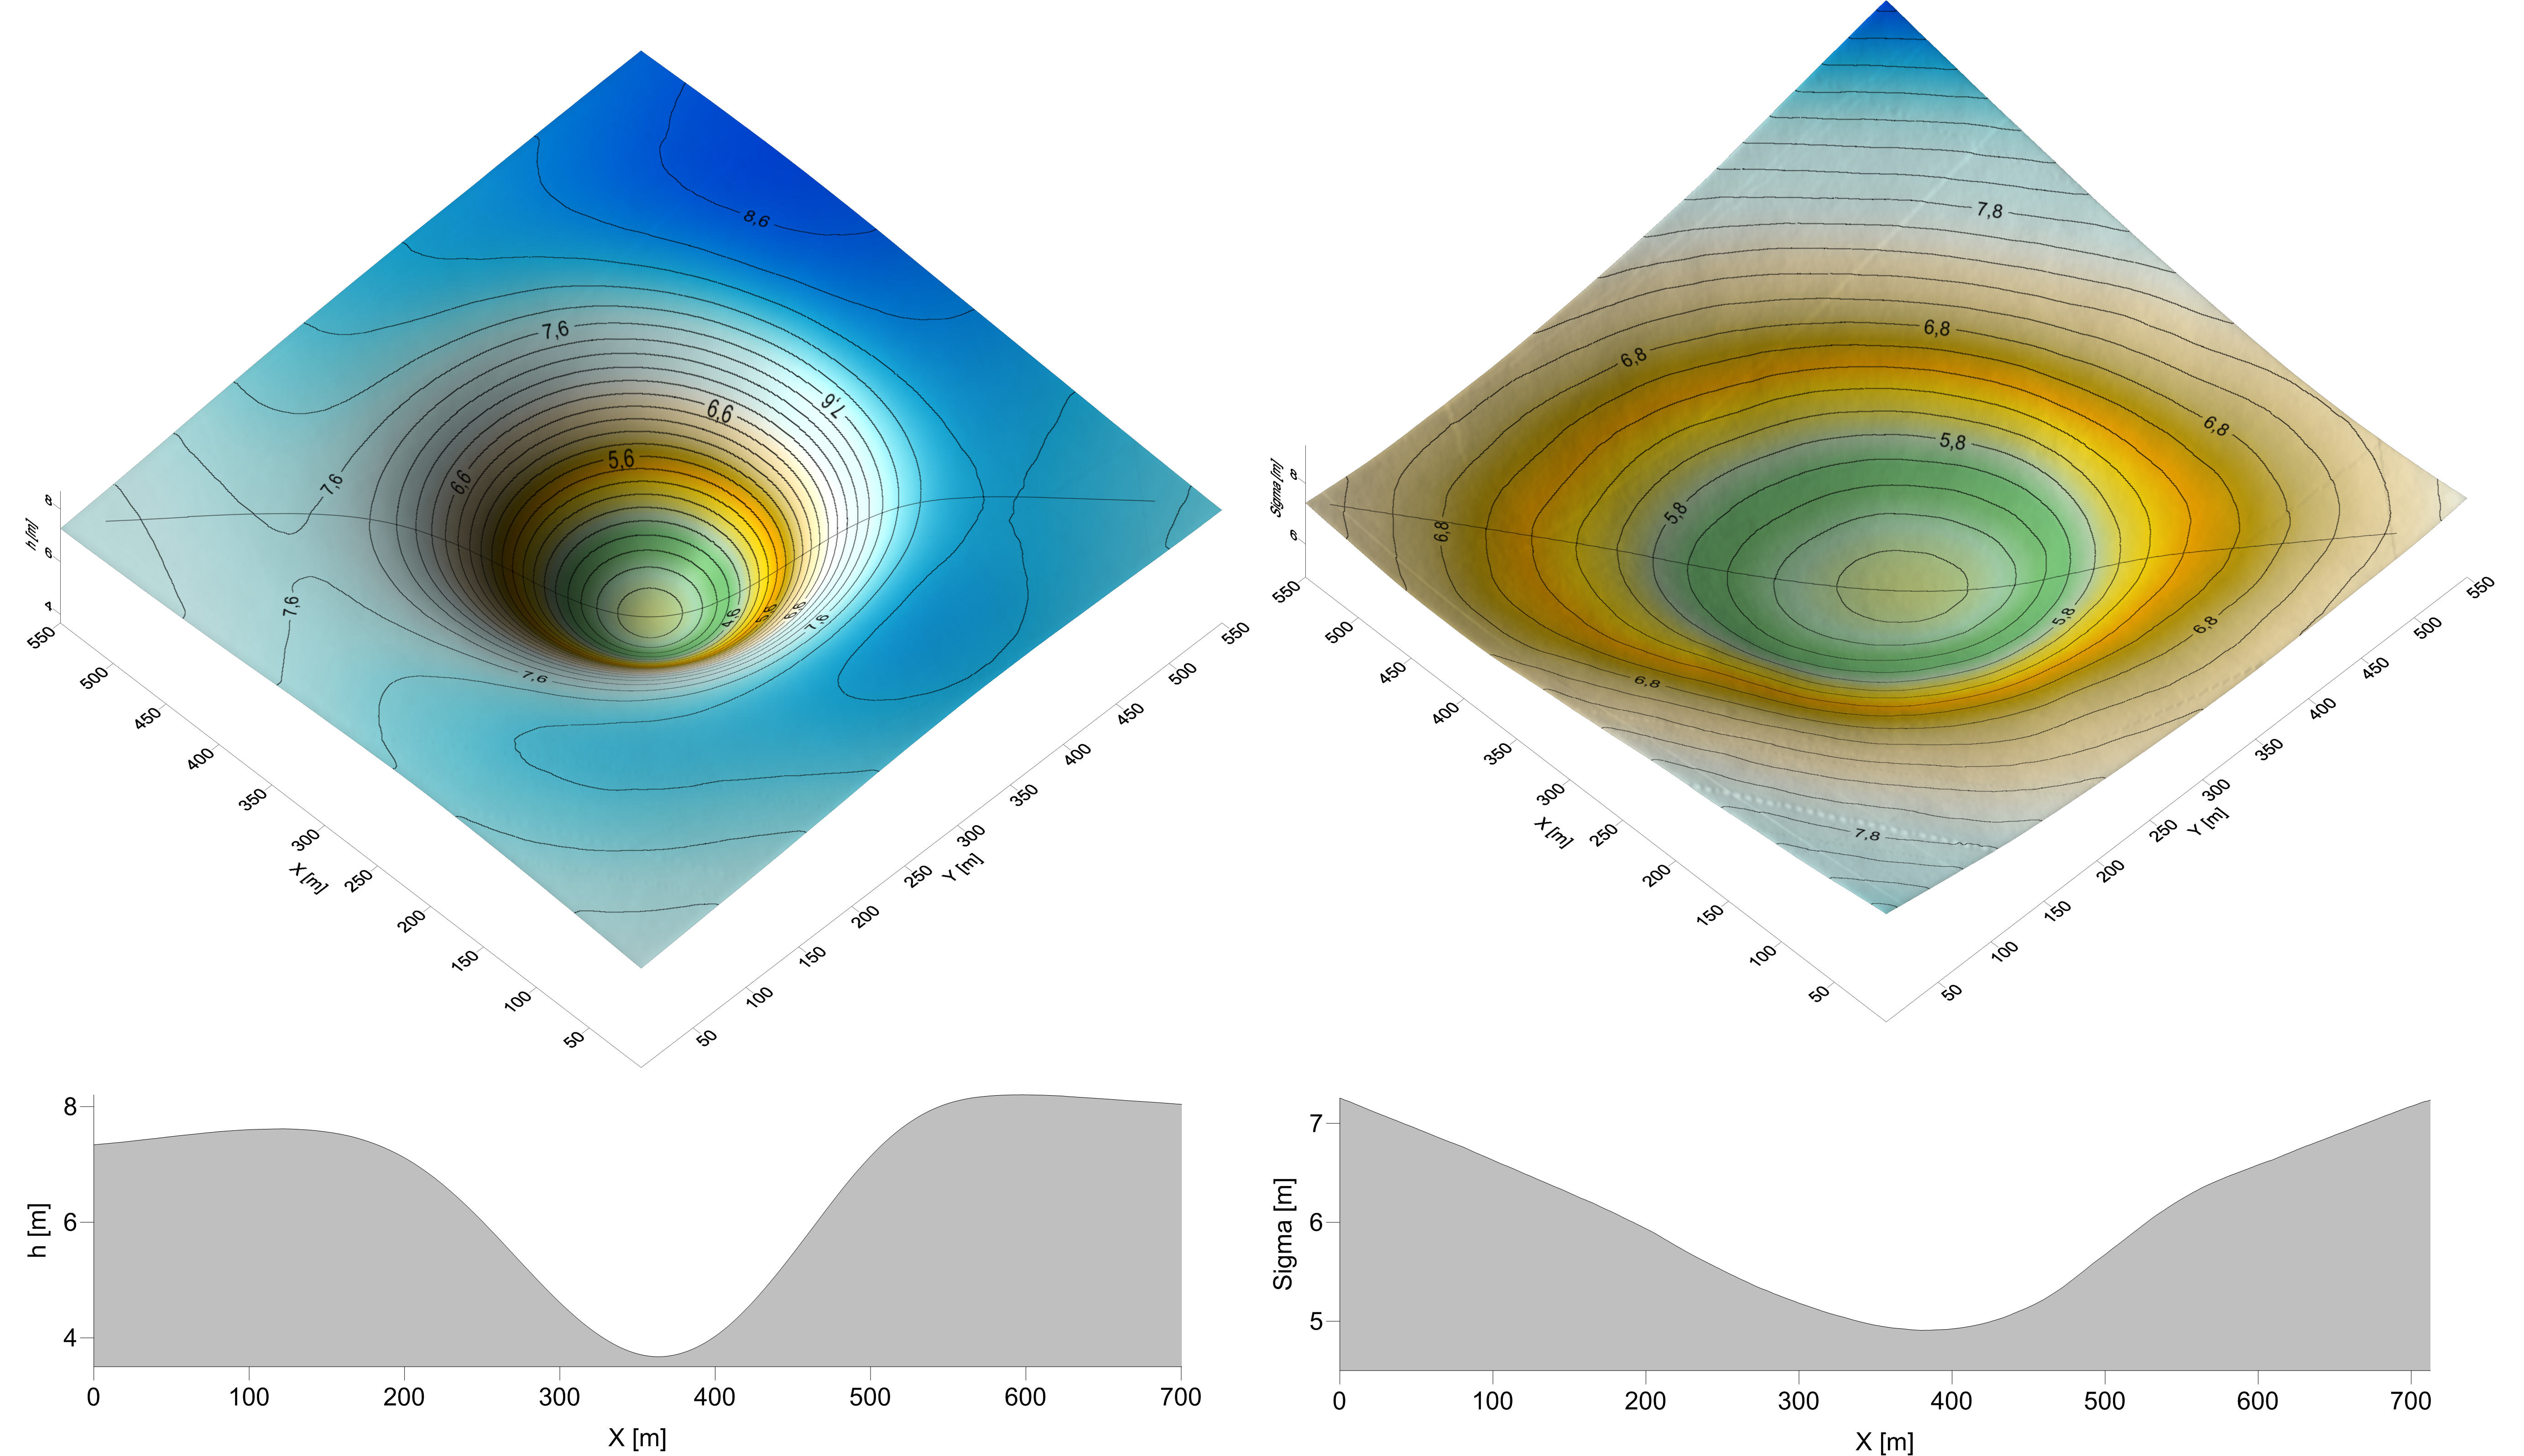
\includegraphics[width=14cm]{slike/menisija-vrtaca-sigma}
    \end{center}
    \caption{Levo: povprečje 8687 realnih vrtač z območja Menišije, pred povprečjem so bile vrtače raztegnjene na velikost največje v setu. Desno: standardna deviacija istega seta vrtač od povprečja.}
    \label{fig:menisija-vrtaca}
  \end{figure}

Na prvi pogled se zdijo dobljeni profili cilindrično simetrični in Gaussove oblike,
\begin{equation}
  h(r,\phi) = A \cdot e^{-\frac{(r-r_0)^2}{\sigma^2}} + C,
  \label{fit-vrtace}
\end{equation}
kjer smo koordinatno izhodišče cilindričnih koordinat postavili v dno vrtače. $\sigma$ nam poda širino, $A$ globino vrtače, $C$ pa jo po $z$ osi umesti na pravo nadmorsko višino. Zaradi cilindrične simetrije funkcija (\ref{fit-vrtace}) ni odvisna od kota $\phi$.

Preidemo v cilindrične koordinate in povprečimo $h(r,\phi)$ po $\phi$:

\begin{equation} 
  \bar h(r) = \frac{1}{2 \pi} \int_0^{2\pi} h(r,\phi) \mathrm{d}\phi.
  \label{povprecenje-phi}
\end{equation}

Tako problem reduciramo na študij profilov vrtač.
Po histogramu (Slika \ref{fig:menisija-polmeri-hist}) vemo, da obstaja velik razred vrtač $23,5m < r_{eff} < 24,5m$. Povprečimo jih po kotu z (\ref{povprecenje-phi}) in nato izračunamo še povprečje njihovih profilov:

\begin{equation} 
  \bar H(r) = \frac{1}{N} \sum_{i} \bar h_i(r).
  \label{povprecenje-profilov}
\end{equation}

Na (Slika \ref{fig:menisija-profil-21-fit}) prikažemo ujemanje $\bar H(r)$ za profile v razredu $23,5m<r_{eff}<24,5m$, s predlagano Gaussovo  funkcijo (\ref{fit-vrtace}). Ujemanje ocenimo za dovolj dobro in nadaljujemo.

  \begin{figure}[h!]
    \begin{center}
      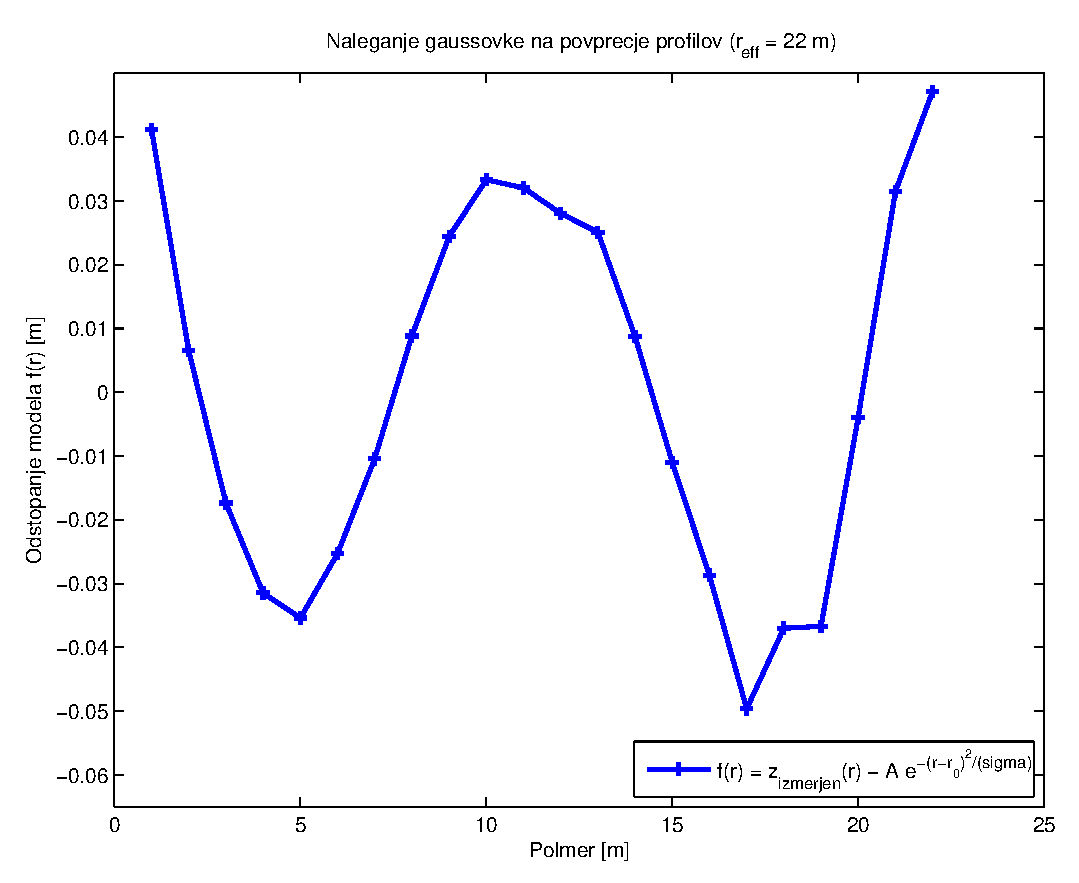
\includegraphics[width=10cm]{slike/menisija-profil-21-fit}
    \end{center}
    \caption{Povprečimo profile vrtač z $r_{eff}=24m$ po (\ref{povprecenje-profilov}), jim prilegamo Gaussovko (\ref{fit-vrtace}) in izrišemo ujemanje prileganja.}
    \label{fig:menisija-profil-21-fit}
  \end{figure}

Ker nam povprečna vrtača (Slika \ref{fig:menisija-vrtaca}) ne pove veliko, nadaljujemo tako, da Gaussovo funkcijo (\ref{fit-vrtace}) nalegamo na prej po enačbi (\ref{povprecenje-phi}) izračunanih profilih realnih vrtač in tako izluščimo parametre $\sigma$ in $A$ realnih vrtač.
Rezultata sta histograma na (Slika \ref{fig:menisija-globine-sigme-hist}).

  \begin{figure}[h!]
    \begin{center}
      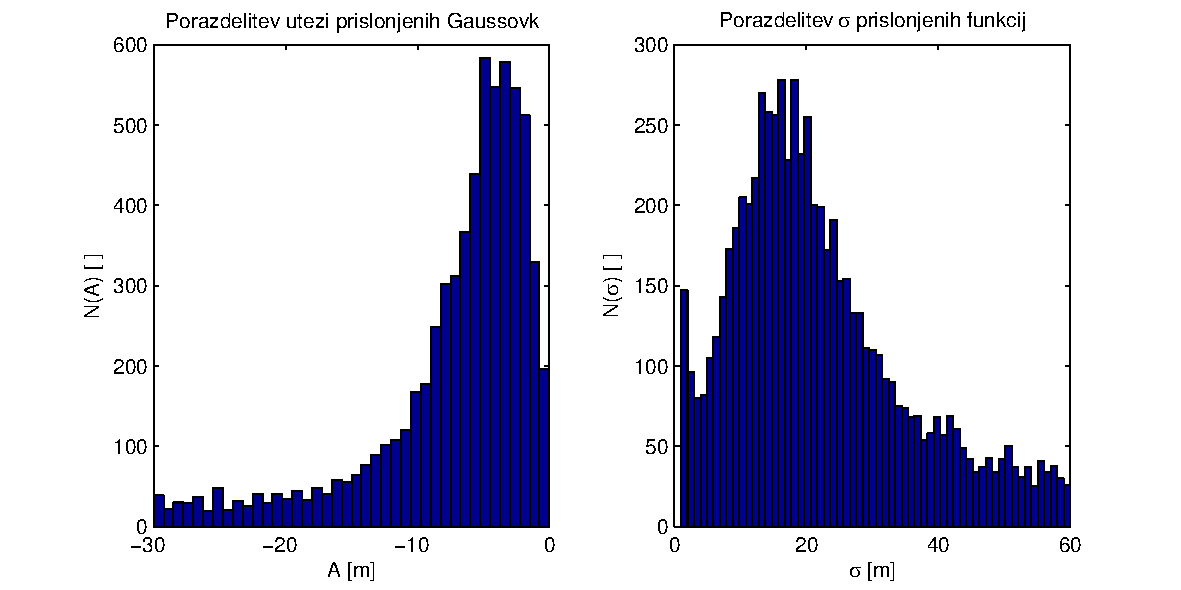
\includegraphics[width=14cm]{slike/menisija-visine-in-sigme-hist}
    \end{center}
    \caption{Vsem najdenim vrtačam prilegamo Gaussovo funkcijo (\ref{fit-vrtace}) in s tem izluščimo parametra A ter $\sigma$. Pridobljene podatke prikažemo na zgornjih histogramih. Izračunamo še povprečji ter standardni deviaciji količin $A$ in $\sigma$: $\bar A= -8,2m$, $\sigma_A=7,7m$, $\bar \sigma=24m$, $\sigma_{\sigma}=13m$.}
    \label{fig:menisija-globine-sigme-hist}
  \end{figure}

Iz vzorca izberemo vrtače tipičnih dimenzij ($5m < r_{eff} < 60m$). Izrišemo odvisnosti $\sigma (r_{eff})$, $A (r_{eff})$ ter $A(\sigma)$ in jim prilegamo linearne funkcije. Rezultat prikažemo na (Slika \ref{fig:menisija-sigma}).

  \begin{figure}[h!]
    \begin{center}
      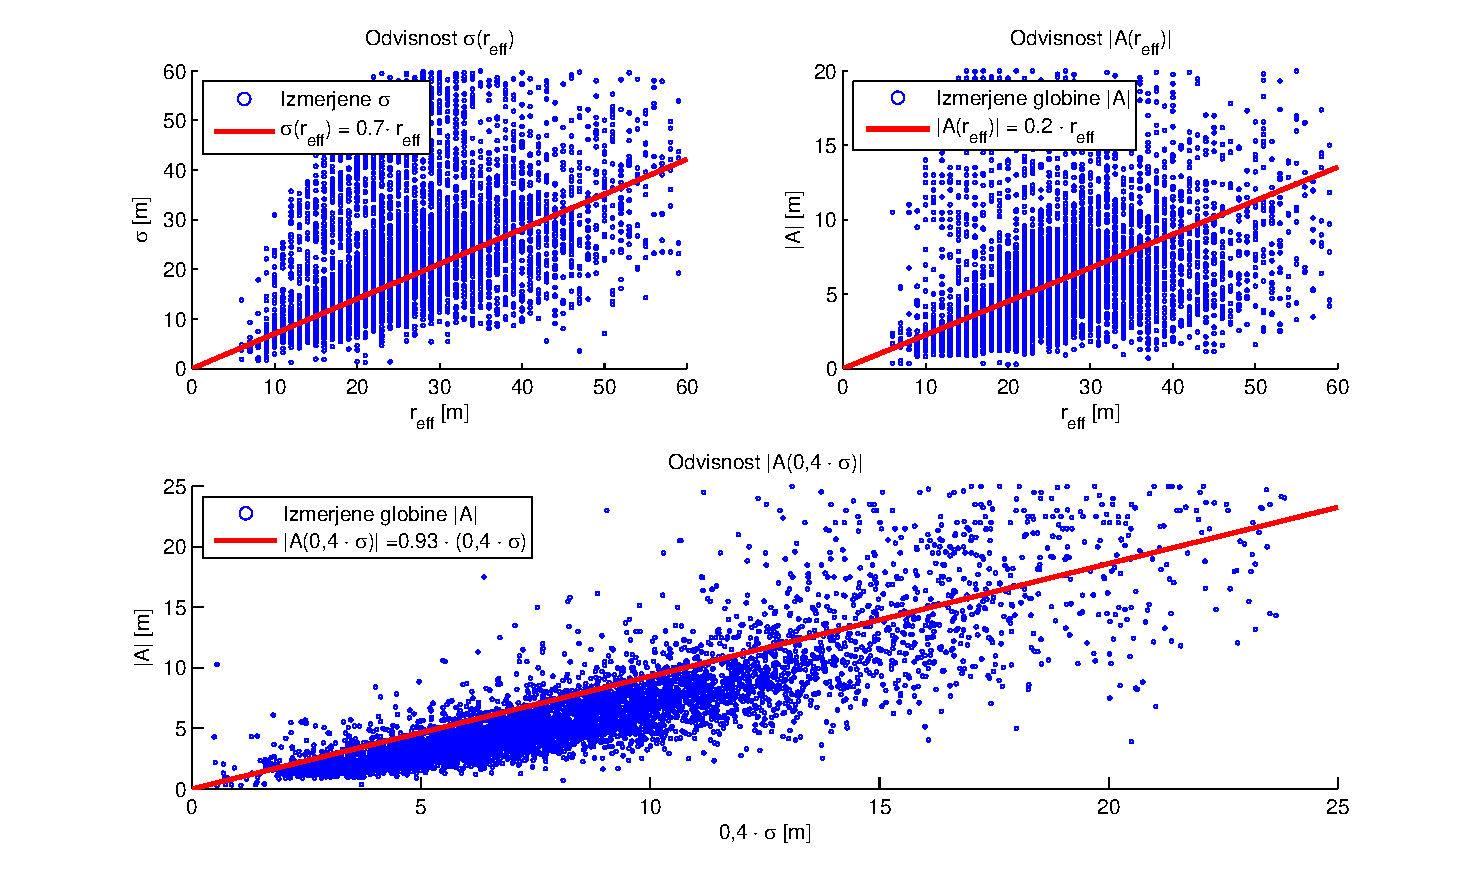
\includegraphics[width=14cm]{slike/menisija-A-sigma-reff}
    \end{center}
    \caption{Iz vzorca izberemo vrtače tipičnih dimenzij ($5m < r_{eff} < 60m$). Izrišemo odvisnosti $\sigma (r_{eff})$, $A (r_{eff})$ ter $A(\sigma)$ in jim prilegamo linearne funkcije. Vidimo, da izrisane odvisnosti niso naključne.}
    \label{fig:menisija-sigma}
  \end{figure}

  Na podlagi teh podatkov težko sklenemo, da (\ref{fit-vrtace}) opiše profil idealne vrtače, a ujemanje je dobro in ga bomo uporabili za analitično modeliranje.

  \begin{figure}[h!]
    \begin{center}
      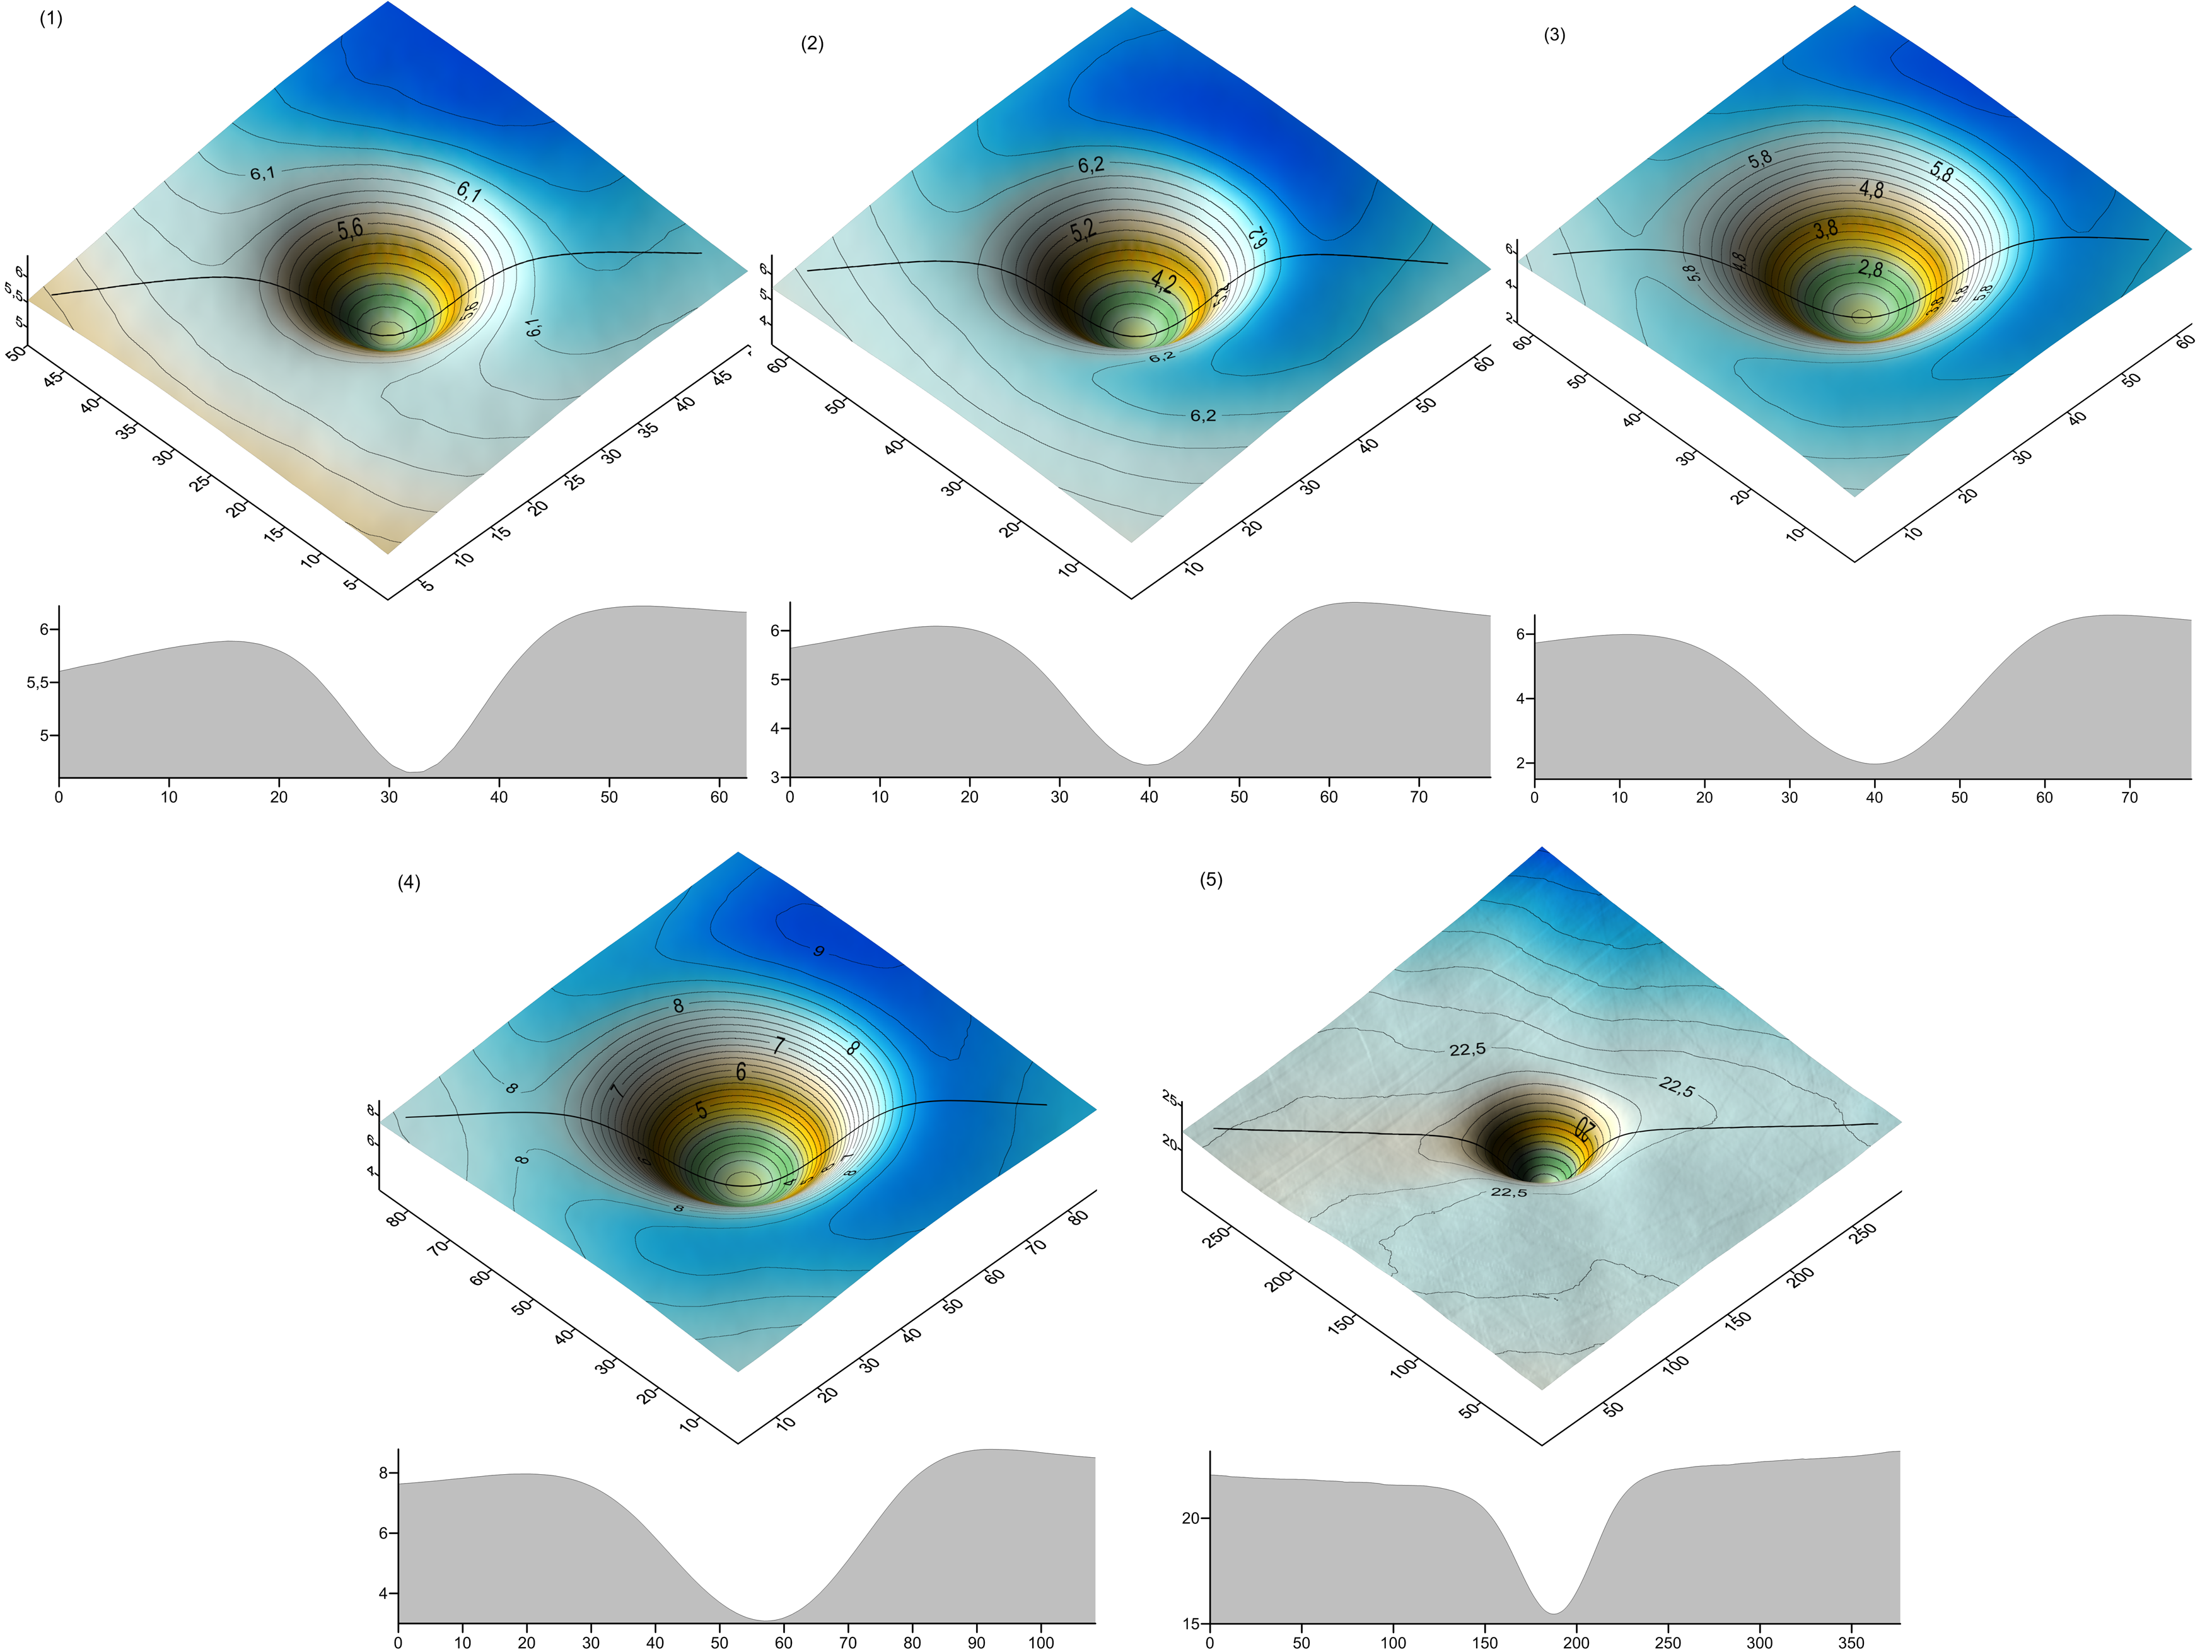
\includegraphics[width=17cm,angle=90]{slike/vrtace-po-razredih-menisija}
    \end{center}
    \caption{Vrtače po velikosti razdelimo v pet razredov (najmanjša petina gre v prvi razred, itn.). Vrtače znotraj razreda tako izrežemo iz površja, da je matrika višinskih točk vrtače vedno enakih dimenzij, pri čemer se vrtača nahaja v sredini. Set vrtač znotraj razredov povprečimo in izrišemo. Dobljeni rezultati so podobni rezultatom povprečenja, pri katerih smo vse vrtače raztegnili na velikost največje v setu: (\ref{fig:menisija-vrtaca}), kar nam da več zaupanja v oba rezultata.}
    \label{fig:menisija-vrtace-po-razredih}
  \end{figure}


  \chapter{Analitično modeliranje vrtač}
  \label{analiticno-modeliranje}

V tem poglavju bomo za opis časovne dinamike vrtač najprej podali definicije potrebne za opis rasti površin in denudacijo kraškega površja analogno modelirali kot stohastično rast površine. Nato bomo podali in komentirali več modelov rasti, ki se skladajo z uvodno tezo, da vrtače nastanejo na ravnem površju in rastejo dokler ne dosežejo stabilne oblike.

  \section{Rast površin}
  \label{definicije}

  V prvem poskusu opisa dinamike vrtač uporabimo definicije s področja rasti površin. Na primeru balističnega usedanja uvedemo potrebne definicije. Delno povzeto po \cite{barabasi1995fractal}.

Balistično usedanje preučuje model, kjer začnemo z ravnim površjem velikosti $L$. Na površje z razdalje večje od najvišje točke na površju in z naključne horizonalne pozicije $x$, padajo kvadratni delčki. Ti navpično padejo na povšje, ter se tam prilepijo. Tak proces pikazuje (Slika \ref{fig:bdep}).
Površje je meja med praznino in naloženimi delčki ter originalnim površjem.

    \begin{figure}[h]
      \begin{center}
        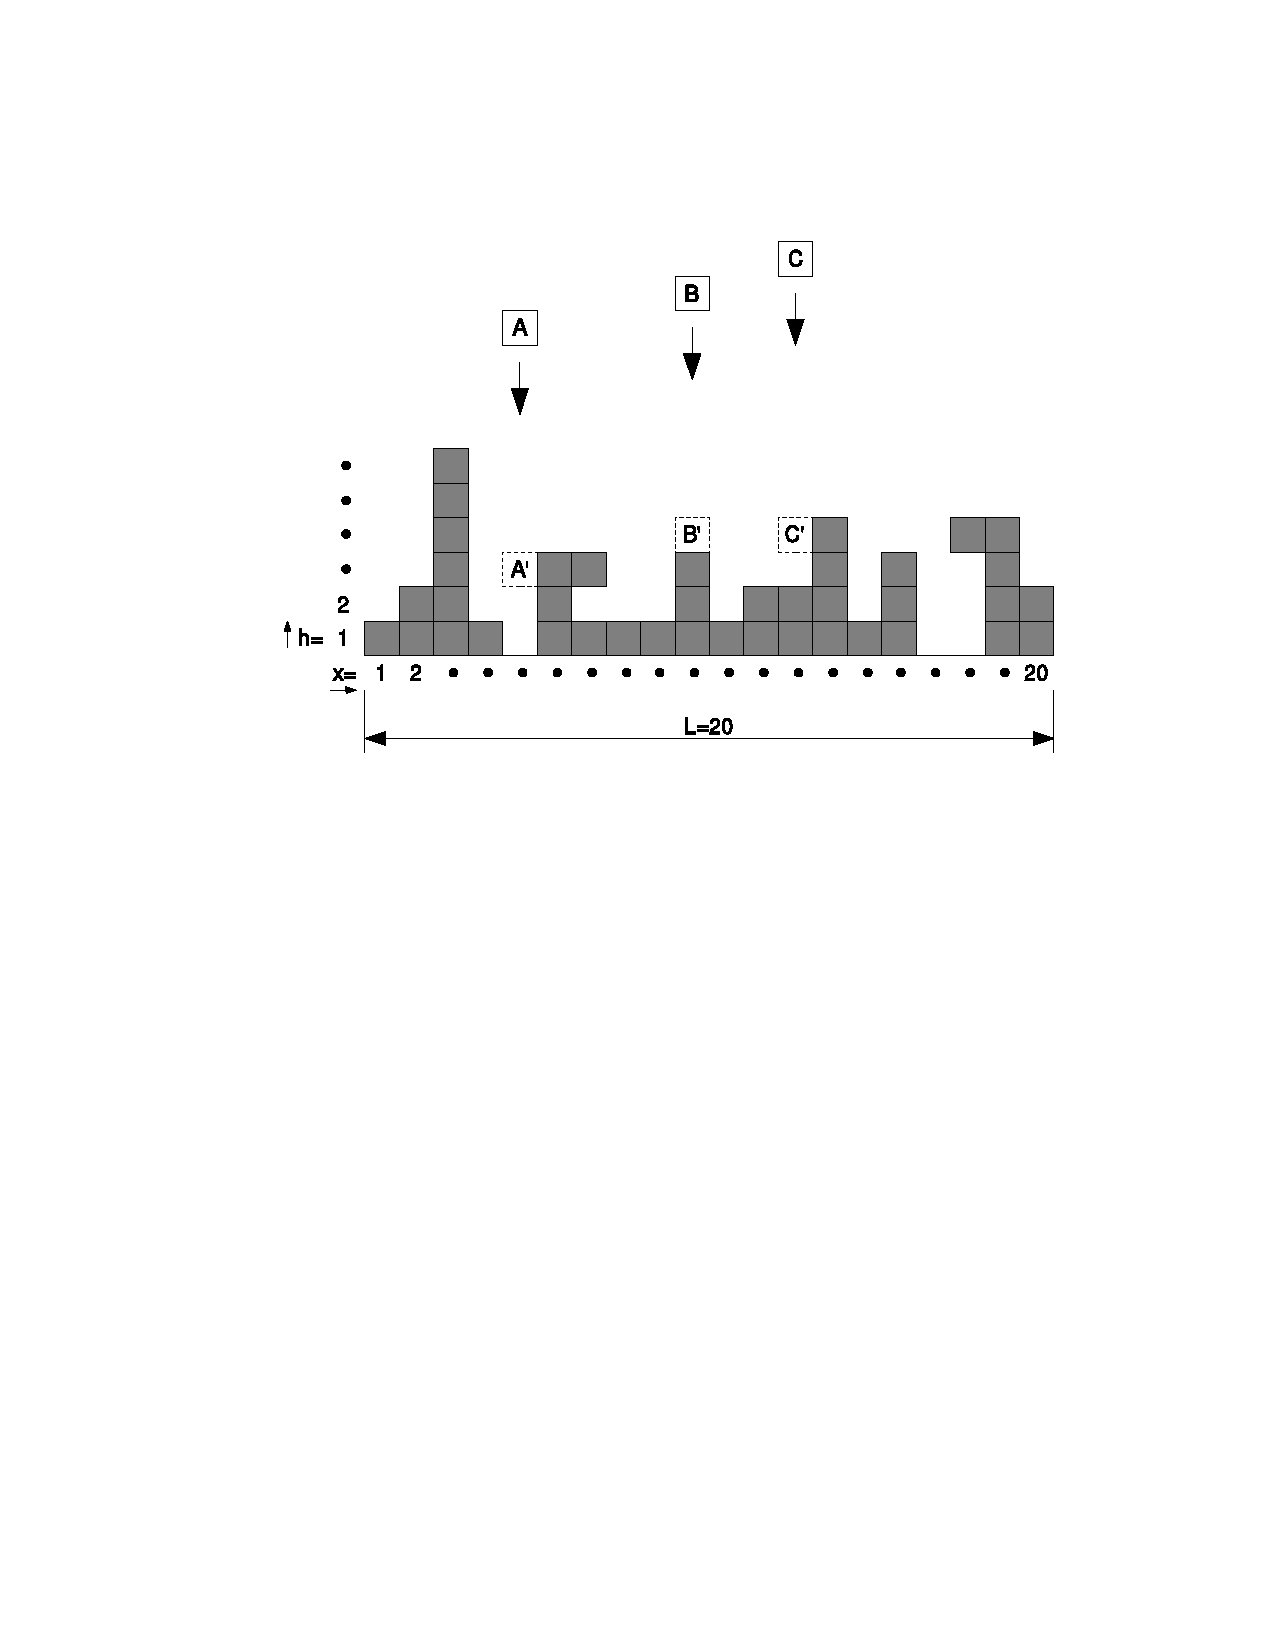
\includegraphics[width=7cm]{slike/bdep}
      \end{center}
      \caption{Skica balističnega nalaganja v eni dimenziji. Delčki A, B in C ob različnih časih $t$ padejo poti površju in se prilepijo na lokacije A’, B’ in C’.}
      \label{fig:bdep}
    \end{figure}

Povprečno višino površja definiramo kot:

  \begin{equation}
    \bar{h} = \frac{1}{L} \sum_{i=1}^L h(i,t),
    \label{povprecna-visina}
  \end{equation}
kjer je $h(i,t)$ višina stolpca $i$ ob času $t$.

Če je usedanje delcev enakomerno porazdeljeno po $x$ in konstantno, se povprečna višina povečuje linearno s časom:

\begin{equation}
  \bar{h}(t) \sim t.
\end{equation}

Širino površja, definiramo s standardnim odklonom višine površja od povprečne višine:

  \begin{equation}
    w(L,t) = \sqrt{\frac{1}{L} \sum_{i=1}^L (h(i,t)-\bar{h}(t))^2}.
    \label{sirina-povrsine}
  \end{equation}

Po definiciji začnemo z ravno površino širine $w(L,t=0)=0$. Kratko prehodno obdobje, ko se delčki lepijo še na ravno podlago imenujemo obdobje Poissonove rasti. V tem obdobju velja: 

\begin{equation}
  w(L,t) \sim t^{1/2}.
\end{equation}

Za tem nastopi obdobje rasti, v katerem velja:
  \begin{equation}
    \begin{array}{lr} w(L,t) \sim t^\beta  & \ t \ll t_s, \end{array}
    \label{beta}
  \end{equation}
kjer je $\beta$ eksponent rasti, ki poda časovno dinamiko hrapavosti površja, $t_s$ pa čas zasičenja.

Po dolgem času rast površja preide v zasičeni režim, v katerem se eksponentna rast širine ustavi in doseže zasičeno vrednost $w_{sat}(L)$, ki je od velikosti sistema $L$ odvisna takole:

  \begin{equation}
    \begin{array}{lr} w(L,t_s) = w_{sat}(L) \sim L^\alpha & (t \gg t_s). \end{array}
    \label{alfa}
  \end{equation}
Eksponent hrapavosti $\alpha$ nam pove kako je hrapavosti zasičenega površja odvisna od njegove velikosti.

Čas zasičenja $t_s$, ob katerem rast površja preide iz nenasičenega v nasičen režim, je odvisen od velikosti površja in je:

  \begin{equation}
    t_s \sim L^z,
    \label{z}
  \end{equation}
kjer je $z$ dinamični eksponent, ki je povezan z dinamiko širjenja površja.

Celotna dinamika širine pri balističnem naleganju je za različne velikosti površja prikazana na (Slika \ref{fig:barabasi}).

    \begin{figure}[h]
      \begin{center}
        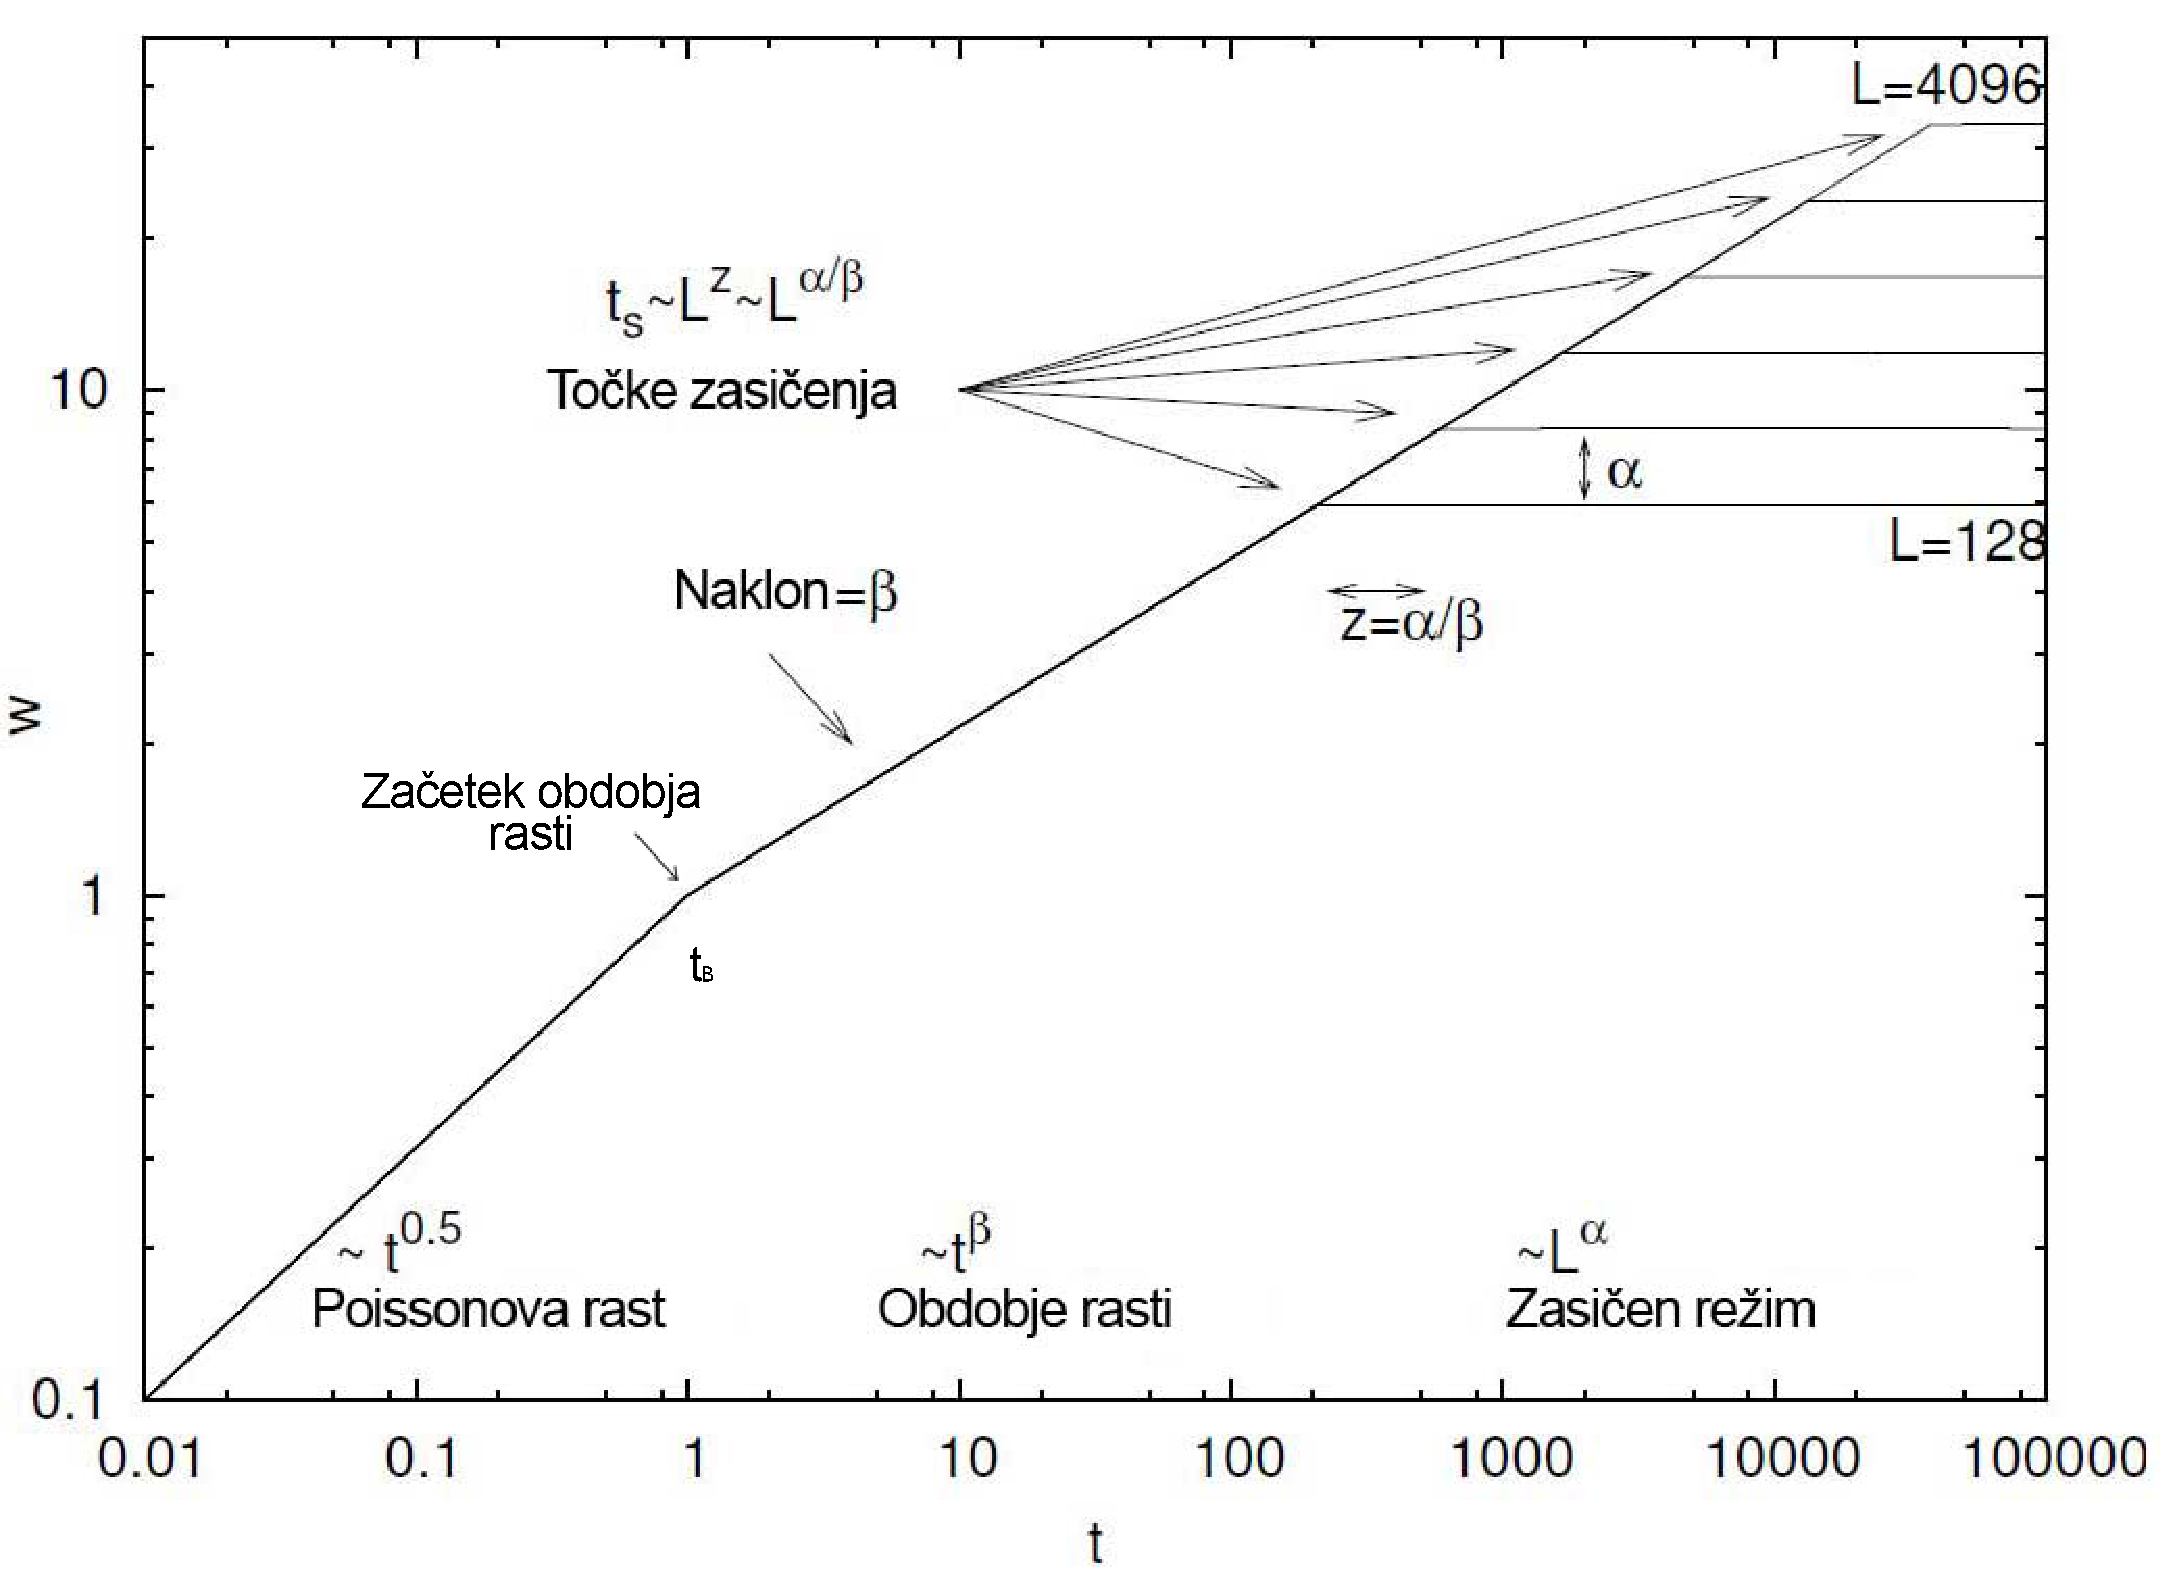
\includegraphics[width=12cm]{slike/bdep3}
      \end{center}
      \caption{Idealni potek širine površja pri balističnem naleganju, za različne velikosti sistema L. Začnemo z ravnim površjem ($w(L,t)=0$) in po kratkem prehodnem obdobju Poissonove rasti ($w(L,t) \sim t^{1/2}$), preidemo v obdobje rasti ($w(L,t) \sim t^{\beta}$). To se zaključi po času $t_s \sim L^z$ in preidemo v zasičen režim ($w(L,t) = w_{sat}(L) \sim L^{\alpha}$). Vir \cite{schwettmann2003}.}
      \label{fig:barabasi}
    \end{figure}

Eksponenti $\alpha$, $\beta$ in $z$ med seboj niso neodvisni.

Iz (Slika \ref{fig:barabasi}) in zveze (\ref{alfa}) vidimo, da se krivulje $w(L,t)/w_{sat}(L)$ zasičijo pri isti konstantni vrednosti, ne glede na velikost sistema $L$.\\
Iz zveze (\ref{z}) pa vidimo, da se bodo širine površij zasitile o istem karakterističnem času $t/t_s$. \\
Sklepamo, da je $w(L,t)/w_{sat}(L)$ funkcija $t/t_s$, torej:

  \begin{equation}
    \frac{w(L,t)}{w_{sat}(L)} \sim f(\frac{t}{t_x}),
  \end{equation}
kjer je $f(t/t_s)$ funkcija lestvičenja. Vstavimo $w_{sat}$ in $t_s$, po zvezah (\ref{alfa}), (\ref{z}) in dobimo Family-Vicsek relacijo lestvičenja:

  \begin{equation}
    w(L,t) \sim L^\alpha f(\frac{t}{L^z}).
    \label{family-vicsek}
  \end{equation}
Za $f(u)$ velja:
  \begin{equation}
    f(u) \propto \left \{ \begin{array}{lr} u^{\beta} & \ u\ll 1 \\
      1 & \ u\gg1\end{array}, \right.
    \end{equation}
kjer je $\beta$ eksponent rasti in $u=\frac{t}{t_s}$.

Sedaj si ogledamo (Slika \ref{fig:barabasi}). Če se točki zasičenja $(t_s,w(t_s))$ približamo z leve, vidimo, da po (\ref{beta}) velja $w(t_s) \sim t_s^\beta$. Hkrati pa, da če se isti točki približamo z desne po (\ref{alfa}) velja $w(t_s) \sim L^\alpha$. Torej $t_s^\beta \sim L^\alpha$ in po (\ref{z}) sledi zakon o lestvičenju:

    \begin{equation}
      z = \frac{\alpha}{\beta}.
    \end{equation}



    \section{Merjenje hrapavosti Menišije}
    \label{hrapavost}

V uvodu smo postavili tezo, da so vse vrtače stare, stabilne oblike. Ko jih opišemo z definicijami rasti površin, domnevamo da so starejše od časa zasičenja ($t_s$) in zanje velja zveza (\ref{alfa}). Predelamo jo v $ w_{sat}=C \cdot L^\alpha $ in dobimo sledečo zvezo za eksponent hrapavosti starega površja:

    \begin{equation}
      \alpha = \frac{\partial ( ln (w_{sat}) ) }{\partial ( ln L )}.
      \label{alpha-numeric}
    \end{equation}

    Na LiDARskem modelu Menišije izračunamo ${w}_{sat}$ za vse mogoče za prereze v smereh sever-jug in vzhod-zahod. Širine površij prerezov $w_{sat}$ nato narišemo v odvisnosti od velikosti prerezov površij $L$.\\
Dobimo graf (Slika \ref{fig:menisija-alfa}), s katerega odberemo, da je $\alpha =  0.409 \pm 0.02$.

\begin{figure}[h]
  \begin{center}
    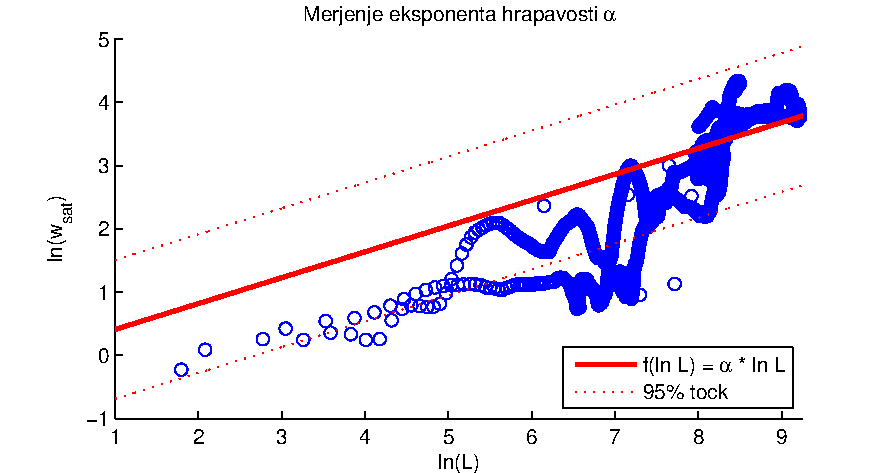
\includegraphics{slike/menisija-alfa.pdf}
  \end{center}
  \caption{Prileganje premice $f(ln(L)) = \alpha \cdot x$ h krivulji $ln(w_{sat}(ln(L)))$ nam poda eksponent hrapavosti $\alpha$.}
  \label{fig:menisija-alfa}
\end{figure}


    \section{Model Kardar-Parisi-Zhang}

    Za modeliranje nastanka vrtač najprej privzamemo, da ima proces poleg stalne hitrosti denudacije kamnine $v$ še stohastično komponento $\eta(\mathbf{x},t)$:
\begin{equation}
  \frac{\mathrm{d} h}{\mathrm{d} t} \bigg|_{denudacija} = v + \eta(\mathbf{x},t),
\end{equation}
kjer $\mathbf{x}$ predstavlja lokacijo na površini ravnine, $v$ povprečno hitrost denudacije, $h(\mathbf{x},t)$ pa višino površine v tej točki ob času $t$. 

Za $\eta (\mathbf{x},t)$ privzamemo, da je časovno in prostorsko nekoreliran šum: 
\begin{equation} 
  \langle \eta(\mathbf{x},t) \rangle=0,
\end{equation}
velja naj tudi:
\begin{equation}
  \langle \eta(\mathbf{x},t) \eta(\mathbf{x'},t')\rangle = 2 D \delta^d(\mathbf{x}-\mathbf{x'})(t-t'),
\end{equation}
kjer je $D$ parameter modela in $d$ število dimenzij prostora.

Taka površina raste kot:
\begin{equation}
  h(\mathbf{x},t) = v \cdot t + \int_0^t \mathrm{d} t' \eta (\mathbf{x},t).
\end{equation}
Zaradi časovne nekoreliranosti šuma $\eta({\mathbf{x},t})$ bi tako površje ohranjalo začetno obliko:

\begin{equation}
  \langle h(\mathbf{x},t) \rangle = v \cdot t.
\end{equation}

Ker je razpadanje kamnine počasen proces in se iz podlage odkrušeni kamni lahko premikajo, privzamemo v naš model še difuzijski člen:
\begin{equation}
  \frac{\mathrm{d} h}{\mathrm{d} t} \bigg|_{difuzija} = \nu \nabla^2 h,
\end{equation}
kjer je $\nu$ utež 'površinske napetosti', ki določa kako močno bo difuzijski člen izravnaval površje.

Končno privzamemo še, da je smer raztapljanja kamnine obrnjena v kamnino, v smeri normale površja (Slika \ref{fig:KPZ}). 
\begin{figure}[h!]
  \begin{center}
    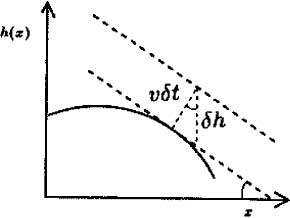
\includegraphics[width=4cm]{slike/KPZ.jpg}
  \end{center}
  \caption{Denudacijo privzamemo v smeri normale površja. $v$ je hitrost denudacije v smeri normale.}
  \label{fig:KPZ}
\end{figure}
\\ Zapišemo Pitagorov izrek za $\delta h$:
\begin{equation}
  \delta h = \sqrt{(v \delta t)^2 + (v \delta t \nabla h)^2} = v \delta t \sqrt{1 + (\nabla h)^2},
  \label{kpz-normala}
\end{equation}
privzamemo $|\nabla h| \ll 1$ in razvijemo (\ref{kpz-normala}) v:
\begin{equation}
  \frac{\partial h}{\partial t} \simeq v + \frac{v}{2} (\nabla h)^2 + \dots.
\end{equation}
Zanemarimo višje člene in zapišemo:
\begin{equation}
  \frac{\partial h}{\partial t} \bigg|_{nelinearno} = v + \frac{v}{2} (\nabla h)^2
\end{equation}

\begin{comment}
    \begin{figure}[h]
      \begin{center}
        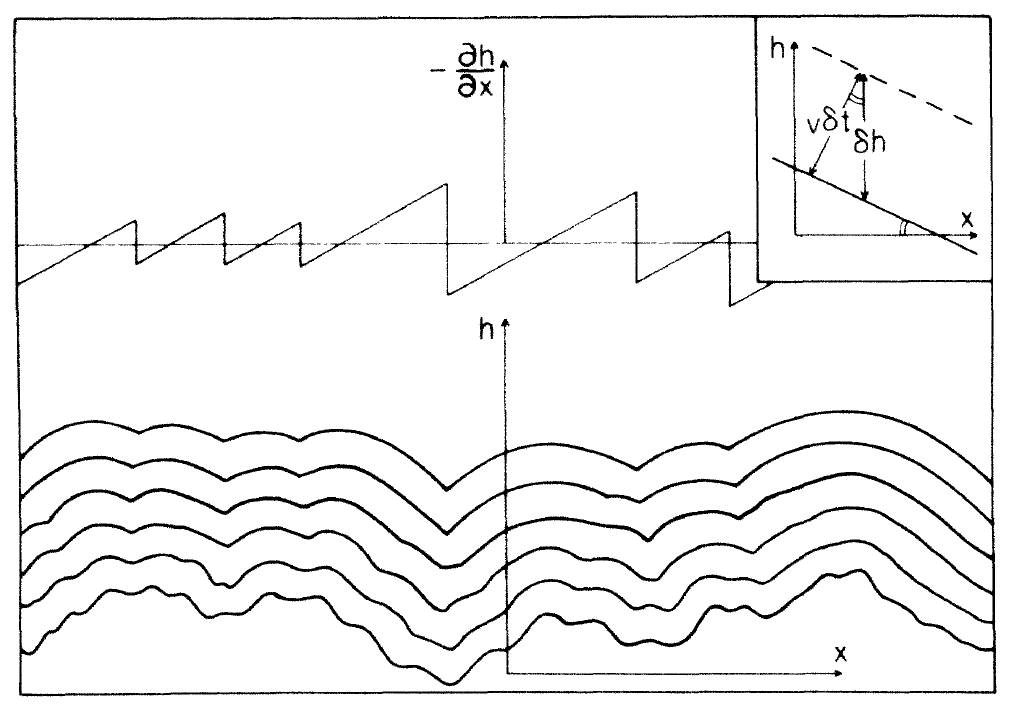
\includegraphics[width=9cm]{slike/kpz.png}
      \end{center}
      \caption{Zaporedni profili deterministične rasti, priraščanje v smeri normale površja je prikazano desno zgoraj.}
      \label{fig:kpz}
    \end{figure}
\end{comment}

Pripravljene člene zdužimo v enačbo, hitrost nelinearnega člena zamenjamo z $\lambda$ $(v \rightarrow \lambda)$:
\begin{equation}
  \frac{\partial h}{\partial t} = \frac{\partial h}{\partial t} \bigg|_{denudacija} + \frac{\partial h}{\partial t} \bigg|_{difuzija} + \frac{\partial h}{\partial t} \bigg|_{nelinearno},
  \label{KPZ1}
\end{equation}
oziroma:
\begin{equation}
  \frac{\partial h}{\partial t} = v + \nu \nabla^2 h + \lambda + \frac{\lambda}{2} (\nabla h)^2 + \eta (\mathbf{x},t).
  \label{KPZ2}
\end{equation}
Postavimo se v premikajoč sistem, ki se premika s hitrostjo $v + \lambda$ v smeri osi $h$ in dobimo Kardar-Parisi-Zhang enačbo (\cite{kardar1986dynamic}):
\begin{equation}
  \frac{\partial h}{\partial t} = \nu \nabla^2 h + \frac{\lambda}{2} (\nabla h)^2 + \eta (\mathbf{x},t).
  \label{KPZ}
\end{equation}
Če vzamemo nastavek:
\begin{equation}
  h(\mathbf{x},t) = \frac{2 \nu}{\lambda} log(Z(\mathbf{x},t)),
\end{equation}
dobimo difuzijsko enačbo v časovno odvisnem naključnem potencialu:

\begin{equation}
  \frac{\partial Z}{\partial t} = \nu \nabla^2 Z + \frac{\lambda}{2 \nu} \eta(\mathbf{x},t) Z,
\end{equation}
katere rešitev je:
\begin{equation}
  h(\mathbf{x},t) = \frac{2 \nu}{\lambda} ln \left( \int_{-\infty}^{\infty} \frac{d^d \xi}{(4 \pi \nu t)^{d/2}} \cdot exp \left[-\frac{(x-\xi)^2}{4 \nu t} + \frac{\lambda}{2 \nu}h(\xi,0) \right] \right).
\end{equation}

    Avtorji \cite{kardar1986dynamic} nato v Fourierovem prostoru s pogojem za beli šum perturbativno rešijo (\ref{KPZ}). Končno pokažejo, da za stohastično priraščanje površja velja: $z = \frac{3}{2}$ in $\alpha=\frac{1}{2}$. To se relativno dobro ujema z $\alpha =  0.409 \pm 0.02$ namerjenim v (Poglavje \ref{hrapavost}).

Da bi kvalitativno ocenili kakšno površje nastane z stohastično denudacijo površja, napravimo preprosto numerično simulacijo. Začnemo z ravnim površjem velikosti $80\times80$ točk, določimo časovni korak $\mathrm{d}t=10^{-3}$ in $10^6$-krat izračunamo:
\begin{equation} 
  h_{i+1} = h_i - dt (\nu \nabla^2 h + \frac{\lambda}{2} (\nabla h)^2 + \eta (\mathbf{x},t)),
\end{equation}
kjer je $h_{i+1}$ nova vrednost v obravnavani točki, $h_{i}$ stara vrednost v obravnavani točki, $\eta (\mathbf{x},t) \in [0,1]$ in določimo $\nu = \lambda = 1$. (Slika \ref{fig:KPZ-numericno}) je primer tako simuliranega površja.

Končno stanje površja pri tem ni statično, med koraki prihaja do manjših premikov. Vendar pa so oblike, ki na površju nastanejo, stabilne ter med seboj podobne po obliki in velikosti.

    \begin{figure}[h]
      \begin{center}
        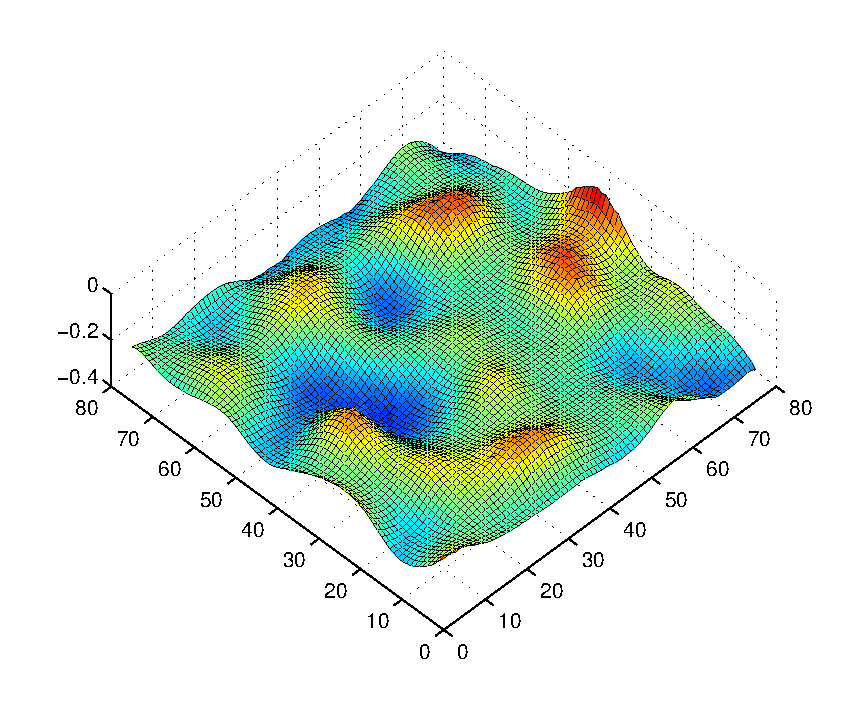
\includegraphics[width=12cm]{slike/KPZ-numericno}
      \end{center}
      \caption{Numerična simulacija po Kardar-Parisi-Zhang enačbi razvijajočega se površja po $10^5$ korakih.}
      \label{fig:KPZ-numericno}
    \end{figure}

\newpage
\section{Reakcijsko-difuzijski model dinamike vrtač}

Do sedaj smo modelirali vrtače kot posledico stohastičnega procesa. Sedaj bomo poskusili modelirati še rast posamezne vrtače. Ker nimamo jasnega modela na katerega bi se oprli je ta problem bolj kompleksen, saj mora v upoštevati vse dejavnike rasti ene same vrtače.
Grobo prevedemo in povzamemo najbolj priznan geomorfološki vir \cite{ford2007karst} (str. 242) ter skico (Slika \ref{fig:vrtaca-ford-williams}), ki konceptualno opišeta dinamiko vrtač:

\begin{quotation}
Skledasta oblika vrtač kaže, da je bilo iz njihovega centra odnešene več kamnine kot z njihovega roba. To nakazuje da je na delu skupen naravni proces, ki fokusira raztapljanje. ... \\
Ko se površje malenkost poglobi, se vzpostavi pozitivna povratna zanka, ki poganja nadaljnje poglabljanje zaradi centripetalnega vodnega toka in posledično korozije. Agresivnost vode se še poveča z biogeno produkcijo $CO_2$ v prsti, ki se ponavadi nabira na dnu depresije. ... \\
Z učinkovitim navpičnim odvajanjem, ki ga omogoči korozijsko razširjanje razpok, se povečuje povprečna hitrost vodnega toka in z njo količina mehansko izprane prsti in kamnine. ... \\
Čeprav je glavna težnja pri nastajanju doline samo ojačitev, imajo nekateri efekti negativen povratni vpliv. Na primer, nekatere prsti, ki pokrivajo kras imajo manjšo prepustnost kot živa skala."
\end{quotation}

\begin{figure}[h!]
  \begin{center}
    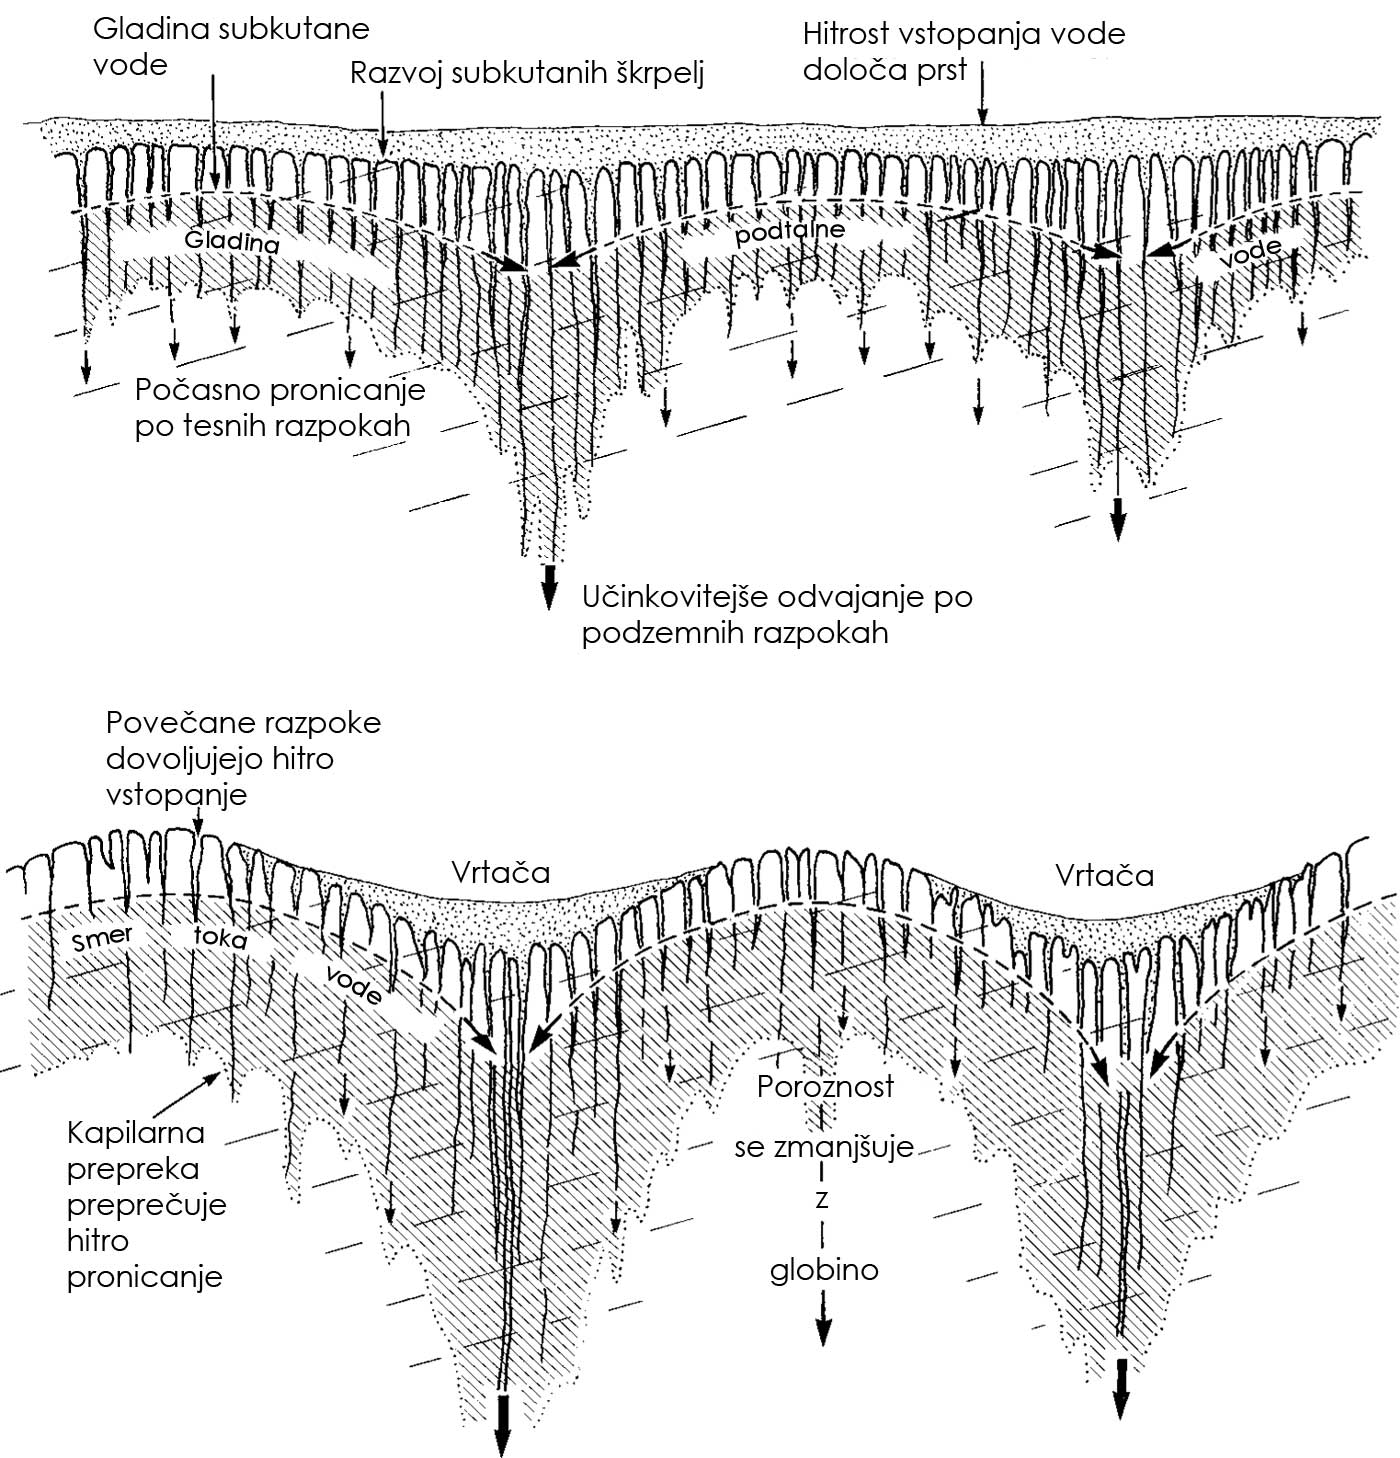
\includegraphics[width=7cm]{slike/vrtaca-ford-williams.jpg}
  \end{center}
  \caption{Geomorfološka skica nastanka vrtač. Na sprva ravnem površju neka začetna točka malenkost bolje odvaja vodo v podzemlje. Zaradi večjega pretoka vode se tam na stiku prsti in kamnine poveča raztapljanje apnenca. Raztapljanje in odnašanje apnenca v podtalnico poglobi površje in s tem poveča lokalno povodje in s tem količino vode odvajane v začetno točko. Dobimo pozitivno povratno zanko in oblikujejo se vrtače. S časom se v vrtačah nabere slabše prepustna prst, odvajanje vode skozi večje razpoke se izboljša, raztapljanje na dnu vrtače zmanjša. To deluje kot negativna povratna zanka. Vir: \cite{ford2007karst}.}
\label{fig:vrtaca-ford-williams}
\end{figure}

Ker mikroskopskega modela take dinamike ne moremo postaviti, si ogledamo nekaj fenomenoloških modelov rasti, ki temeljijo na reakcijsko-difuzijski dinamiki (\ref{dinamicna-splosna}) opisa rasti, ki je primeren za opis prostorsko porazdeljenih kemijskih reakcij. Ti modeli predpostavijo, kako na neko količino neke vpliva izbrana deterministična dinamika in difuzija.

\begin{equation}
  \frac{ \partial h(t,x) }{ \partial t} = D \Delta h + F(h).
  \label{dinamicna-splosna}
\end{equation}

Najprej ločeno pogledamo različne variacije determinističnega člena $F(h)$ za (\ref{dinamicna-splosna}). Izbor je povzet po \cite{kandler2010population}.

\begin{comment}
    \begin{equation}
      F(h) = \left \{ \begin{array}{lr} 
        a \cdot h \\
        a \cdot h \cdot (1 - \frac{h}{K}) \\
        a \cdot (K - h) \\
        - h \cdot e^{-a t}
      \end{array}. \right. 
      \label{dinamicna-variacije}
    \end{equation}
\end{comment}

    \subsection{Eksponentna rast}

    V modelu eksponentne rasti predpostavimo, da je rast sorazmerna z vrednostjo ($h(t)$) v izbrani točki. Dobimo enačbo (\ref{dinamicna-eksponentna}), ki jo reši funkcija (\ref{dinamicna-eksponentna-resitev}), in jo pri variaciji parametra $a$ narišemo (Slika \ref{fig:eksponentna-rast}).

    \begin{equation}
      \frac{\partial h(t)}{\partial t} = a \cdot h(t).
      \label{dinamicna-eksponentna}
    \end{equation}

    \begin{equation}
      h(t) = h_0 e^{a t}.
      \label{dinamicna-eksponentna-resitev}
    \end{equation}

    \begin{figure}[h]
      \begin{center}
        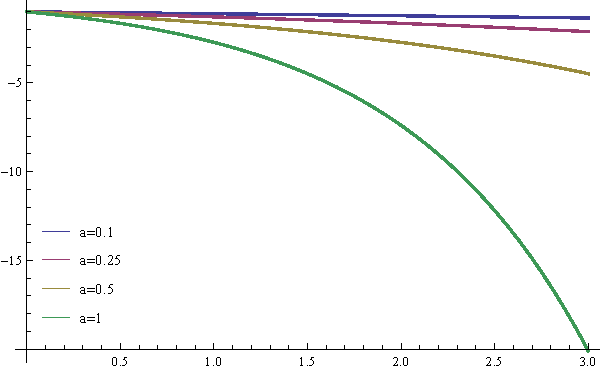
\includegraphics[width=10cm]{slike/eksponentna-rast}
      \end{center}
      \caption{Vzeli smo začetno vrednost $h_0 = -1$ in variirali vrednost $a$. \newline $a=0,1;0,25;0,5;1$.}
      \label{fig:eksponentna-rast}
    \end{figure}

    Če je parameter $a > 0$, bomo vedno dobili neomejeno rast, kar zmanjšuje splošnost tega modela. Vseeno pa je v omejenih intervalih uporaben za npr. opis rasti populacij držav, širjenje virusov, jedrskih verižnih reakcij, itn. Uporabnost modela se konča, ko se sistem zasiti - to je, ko zmanjka virov, ki rast poganjajo (če gledamo dane primere - ko zmanjka hrane, celic, jeder).
    Pri vrtačah je možno, da imamo eksponentno rast v začetku, a tega ne moremo ne dokazati ne ovreči. Vsekakor pa je ni v ravnovesni fazi, saj zelo globokih vrtač ne opazimo.


    \subsection{Logistična rast}

    V model logistične rasti predpostavimo, da je rast sorazmerna z višino v izbrani točki, ter da se zmanjšuje, ko se približujemo fizikalnim omejitvam sistema (npr. pomanjkanju hrane, življenjskega prostora, itn). To zapišemo v enačbo (\ref{dinamicna-logisticna}), ki jo reši funkcija (\ref{dinamicna-logisticna-resitev}).

    \begin{equation}
      \frac{\partial h(t)}{\partial t} = a \cdot \left( 1 - \frac{h(t)}{K} \right) h(t).
      \label{dinamicna-logisticna}
    \end{equation}

    \begin{equation}
      h(t) = \frac{h_0 K e^{a t}}{K + h_0 (e^{a t}-1)}.
      \label{dinamicna-logisticna-resitev}
    \end{equation}

    \begin{figure}[h]
      \begin{center}
        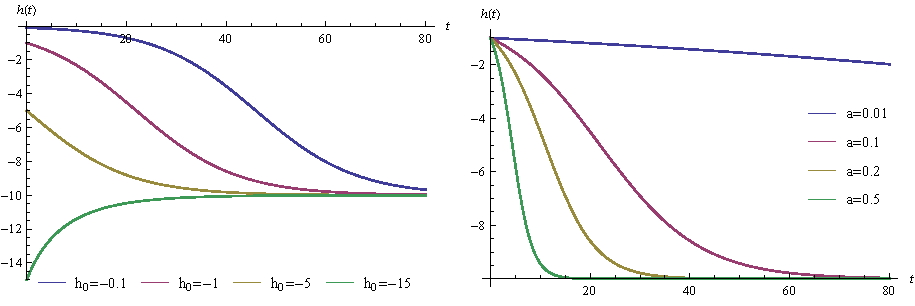
\includegraphics[width=14cm]{slike/logisticna-rast}
      \end{center}
      \caption{Logistična rast po (\ref{dinamicna-logisticna-resitev}). Vzeli smo $K=-10$ in variirali ostale parametre. V prvem primeru smo pri $a=0,1$ vzeli $h_0=-0,1;-1;-5;-15$. V drugem pa pri $h_0=-1$, $a=0.01;0.1;0.2;0,5$.}
      \label{fig:logisticna-rast}
    \end{figure}

    Vidimo, da ne glede na izbiro začetne točke $h_0$, vrednost h(t) konvergira proti vrednosti $K$. Torej je rast omejena s kapaciteto sistema K.
    Če funkcijo (\ref{dinamicna-logisticna-resitev}) Taylorjevo razvijemo, vidimo, da je rast, kjer $h(t) \ll K$, približno $a h(t)$. V območju, kjer je $h(t)$ bližji $K$, pa postane drugi člen v razvoju $-a h(t)^2 / K$ pomembnejši in rast se po dolgem času ustavi.
    Model logistične rasti se uporablja za modeliranje človeških in živalskih populacij, rasti tumorjev, širjenje inovacij v družbi in sprememb v jeziku. Zaradi omejene rasti pa se zdi tudi zanimiv kandidat za modeliranje dinamike vrtač.


    \subsection{Omejena eksponentna rast}

    Model omejene eksponentne rasti pravi, da je rast tem večja, čim dlje smo od omejitve sistema $K$ in vedno v smeri proti vrednosti $K$. To zapišemo v enačbo (\ref{dinamicna-omejena-eksponentna}) in rešimo z (\ref{dinamicna-omejena-eksponentna-resitev}).

    \begin{equation}
      \frac{\partial h(t)}{\partial t} = a \cdot ( K - h(t) ) = a K - a h(t).
      \label{dinamicna-omejena-eksponentna}
    \end{equation}

    Rešitev pa je
    \begin{equation}
      h(t) = K - (K - h_0) e^{-a t}.
      \label{dinamicna-omejena-eksponentna-resitev}
    \end{equation}

    Medtem ko je omejena eksponentna rast podobna logistični, pa ima logistična v začetku položnejšo rast. Omejena eksponentna rast se uporablja za modeliranje sistemov, v katerih dinamiko poganjajo zunanji dejavniki in znotraj katerih ni interakcij. Naprimer pri širjenju inovacij v družbi.

    \begin{figure}[h]
      \begin{center}
        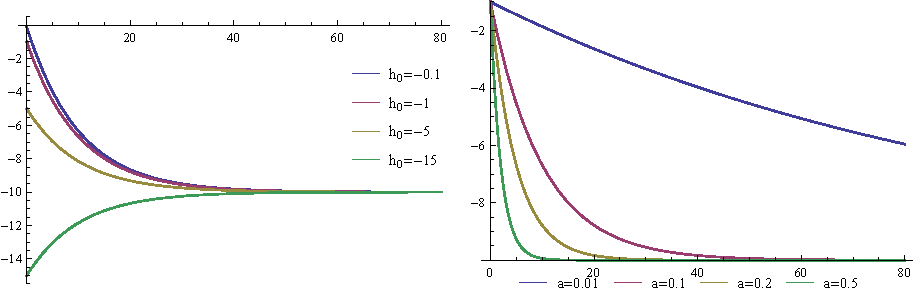
\includegraphics[width=14cm]{slike/omejena-eksponentna-rast}
      \end{center}
      \caption{Omejena eksponentna rast po (\ref{dinamicna-omejena-eksponentna-resitev}). Vzeli smo $K=-10$ in variirali ostale parametre. V prvem primeru smo pri $a=0,1$ vzeli $h_0=-0,1;-1;-5;-15$. V drugem pa pri $h_0=-1$, $a=0.01;0.1;0.2;0,5$.}
      \label{fig:omejena-eksponentna-rast}
    \end{figure}



    \subsection{Gompertzova rast}

    Pri modelu Gompertzove rasti vzamemo, da se faktor rasti s časom spreminja po enačbi (\ref{dinamicna-gompertzova-faktor}), kar nam da enačbo (\ref{dinamicna-gompertzova}) in rešitev (\ref{dinamicna-gompertzova-resitev}), iz katere lahko dobimo še asimptotsko rešitev (\ref{dinamicna-gompertzova-faktor}), ki je podobna zasičenosti modela pri prejšnjih dveh primerih, a nastopi zaradi postopnega prenehanja rasti, in ne zaradi povratne zanke (kot v primeru logistične in omejene eksponentne rasti).

    \begin{equation}
      a(t) = a_0 \cdot e^{- k t}.
      \label{dinamicna-gompertzova-faktor}
    \end{equation}
    \begin{equation}
      \frac{\partial h(t)}{\partial t} = a(t) \cdot h(t) = a_0 e^{ -k t} h(t).
      \label{dinamicna-gompertzova}
    \end{equation}
    \begin{equation}
      h(t) = h_0 \cdot e^{\frac{a_0}{k}(1-e^{-kt})}.
      \label{dinamicna-gompertzova-resitev}
    \end{equation}
    \begin{equation}
      h(t) = h_0 \cdot e^{\frac{a_0}{k}} \quad \text{pri} \quad t \rightarrow \infty.
      \label{dinamicna-gompertzova-limita}
    \end{equation}

    \begin{figure}[h!]
      \begin{center}
        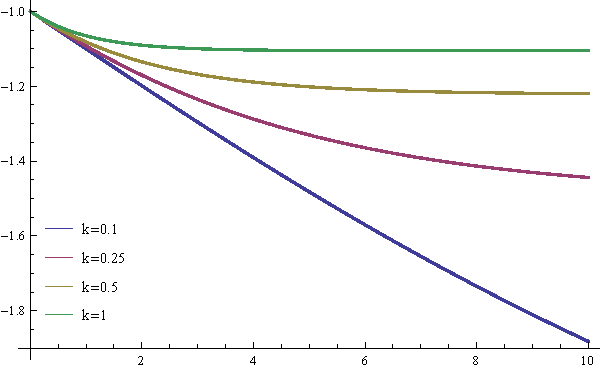
\includegraphics[width=10cm]{slike/gompertzova-rast}
      \end{center}
      \caption{Vzeli smo $h_0=-1$ in $a_0=0,1$ in variirali $k=0,1;0,25;0,5;1$.}
      \label{fig:gompertzova-rast}
    \end{figure}
[TODO]Opis razlik in podobnosti med temi modeli deterministične dinamike[TODO]

    \section{Difuzijsko modeliranje dinamike vrtač}

V prejšnjem poglavju predlagane deterministične nastavke dinamike sedaj zaporedno vstavljamo v splošno reakcijsko-difuzijsko enačbo (\ref{dinamicna-splosna}) in jo numerično rešujemo pri robnih pogojih (\ref{rd-robni}). Rešitve prikažemo in komentiramo njeno časovno dinamiko. Izbrani robni pogoji

    \begin{equation}
      \begin{aligned}
        h(0,x) =  - e^{-x^2}, x \in D \\
        h(t,x) = 0, x \in \partial D \\
        \frac{\partial h(t,x)}{\partial n} = 0, x \in \partial D
      \end{aligned}
\label{rd-robni}
    \end{equation}
postavijo, da začnemo na ravni podlagi, z majhno udrtino Gaussove oblike. Vrednost $h(t,x)$ in njen prvi odvod po normali na robu območja postavimo na $0$.

    \subsection{Eksponentna rast}

    \begin{equation}
      \frac{ \partial h(t,x) }{ \partial t} = D \Delta h(t,x) + a \cdot h(t,x).
      \label{difuzija-eksponentna-rast}
    \end{equation}

    Sistem nam da eksponentno rast, kot je prikazano na (Slika \ref{fig:difuzija-eksponentna-rast}).

    \begin{figure}[h!]
      \begin{center}
        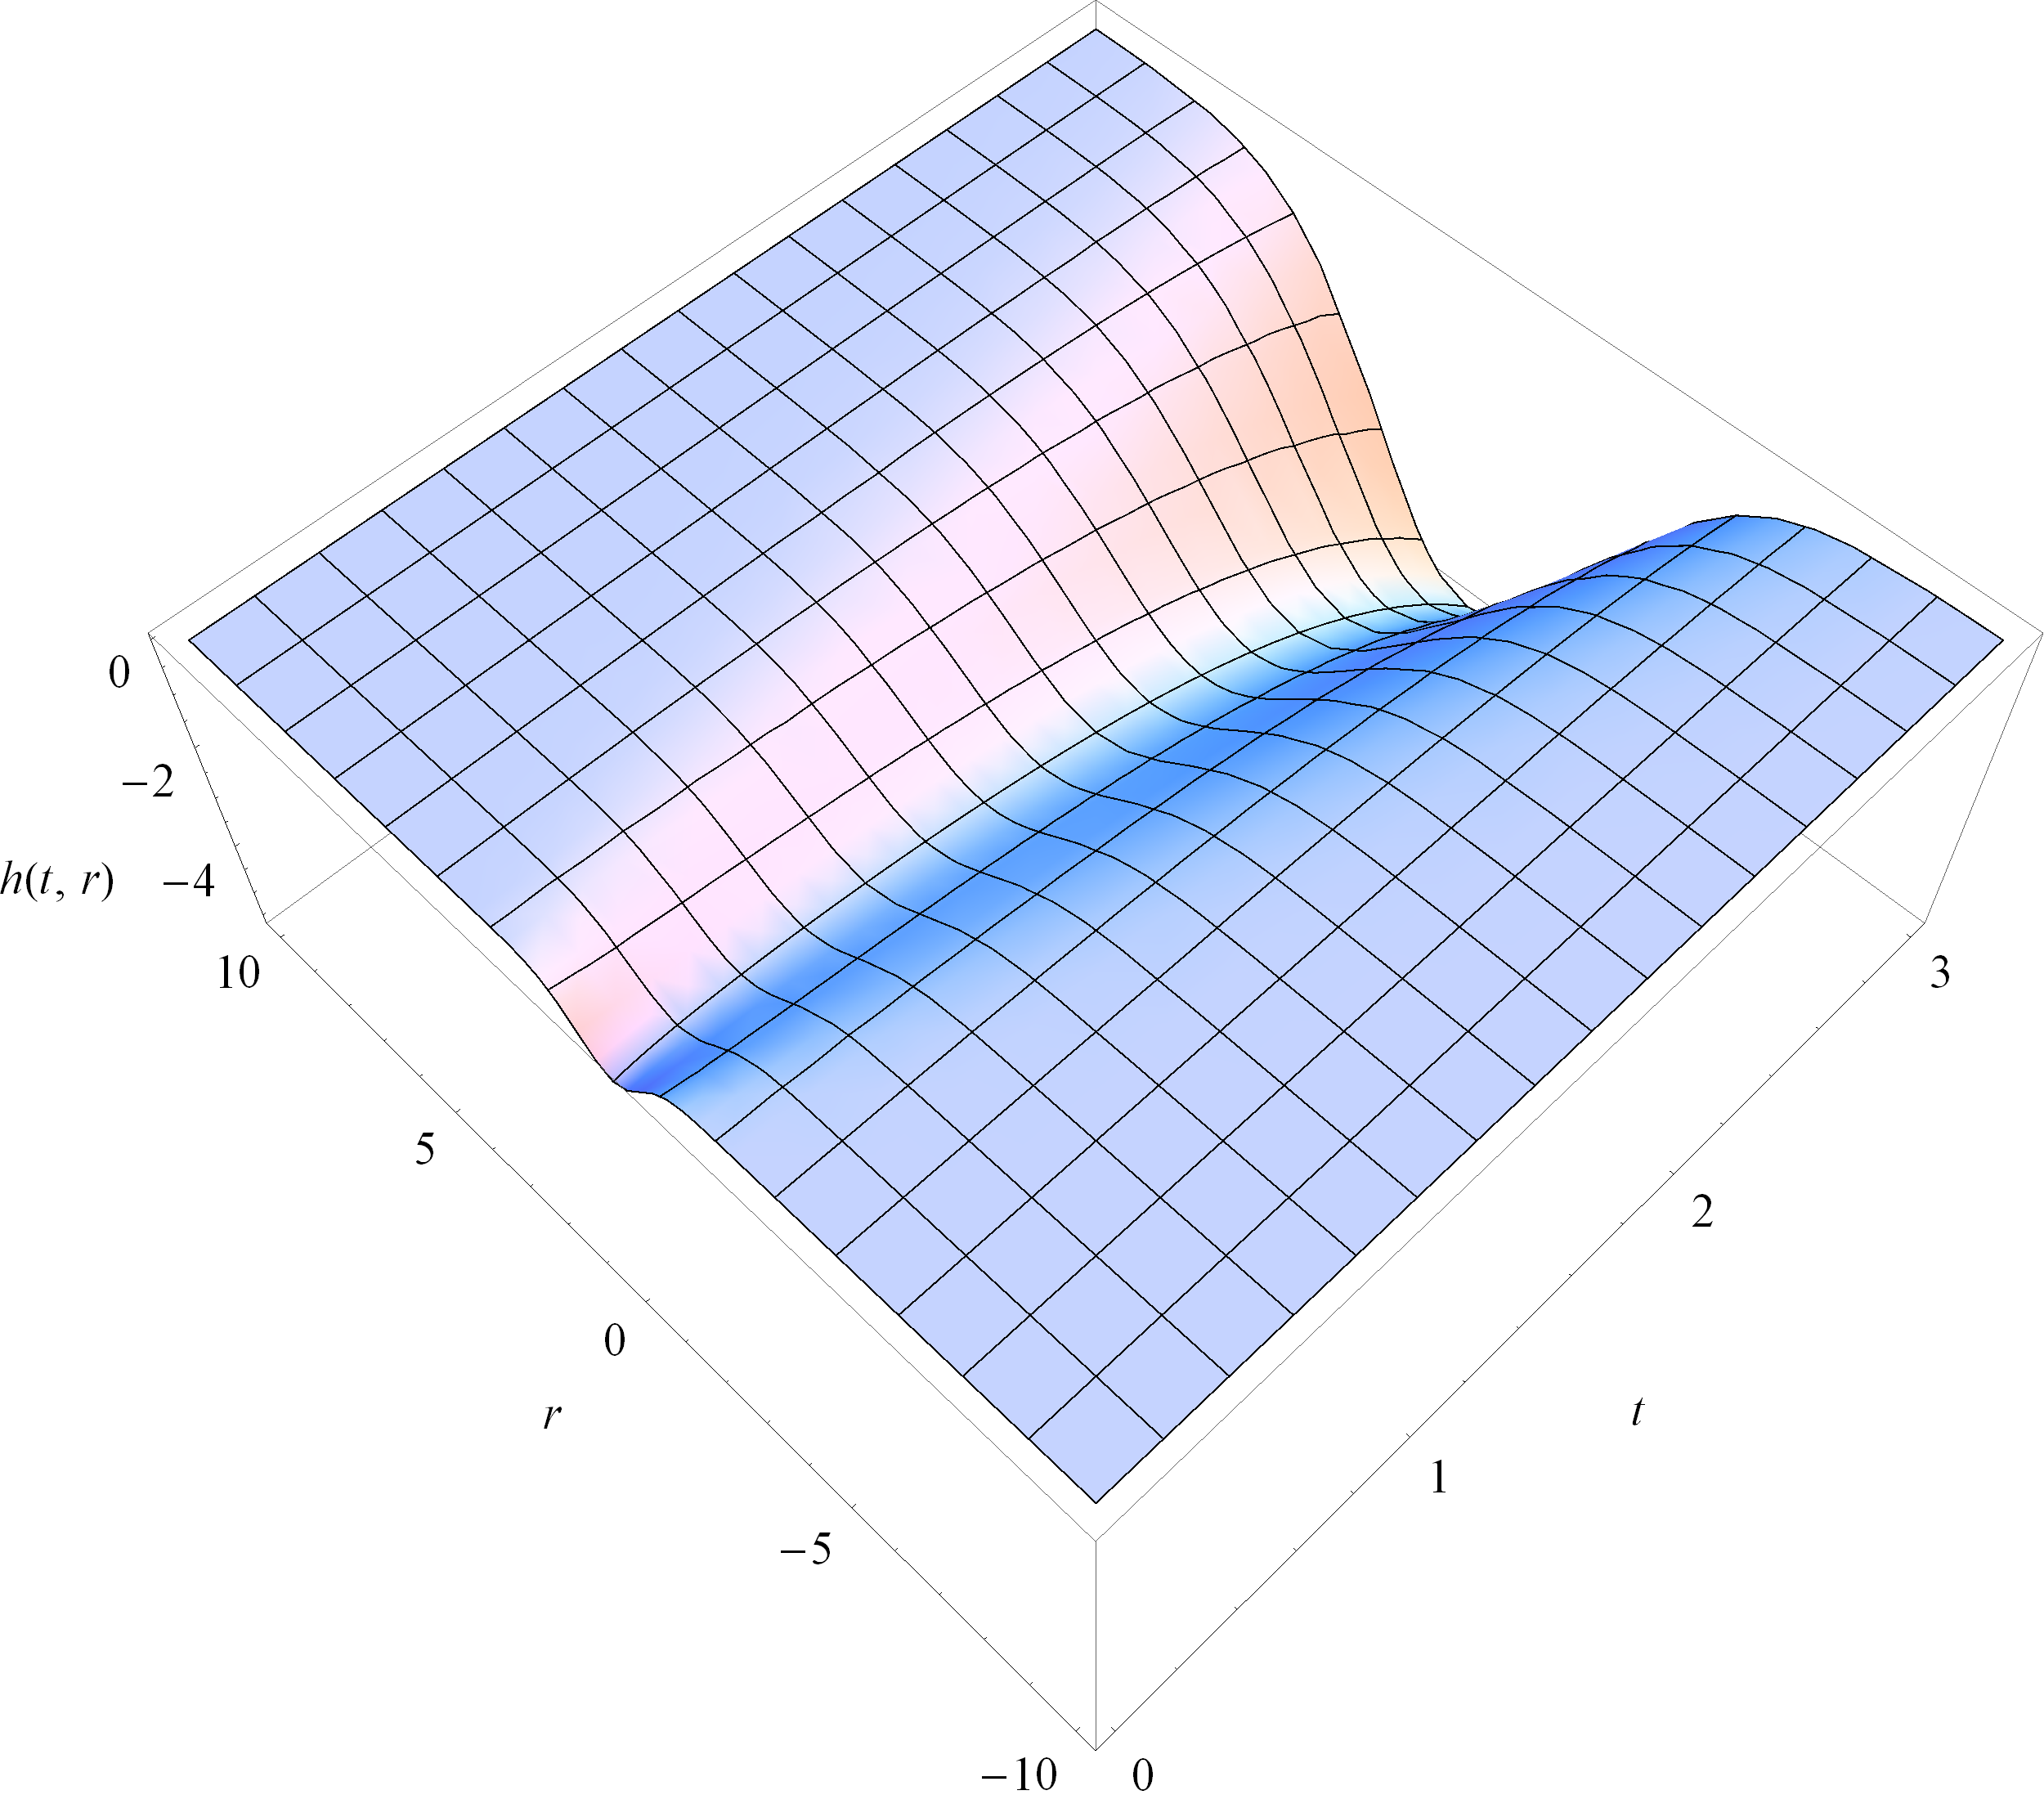
\includegraphics[width=9cm]{slike/difuzija-eksponentna-rast2}
      \end{center}
      \caption{Vzeli smo $D=1$, $a=1$.}
      \label{fig:difuzija-eksponentna-rast}
    \end{figure}

[TODO]Kdaj je to primeren mode. Primeri.[TODO]

Eksponentna rast za vrtače ni primeren model, saj zelo velikih vrtač v naravi ne opazimo.

    \subsection{Logistična rast}
[TODO]Več opisa.[TODO]
    Dobimo t.i. Fisher-Kolmogorovo enačbo:

    \begin{equation}
      \frac{ \partial h(t,x) }{ \partial t} = D \Delta h(t,x) + a \cdot h(t,x) \cdot (1 - \frac{h(t,x)}{K}).
      \label{difuzija-logisticna-rast}
    \end{equation}
    \begin{figure}[h!]
      \begin{center}
        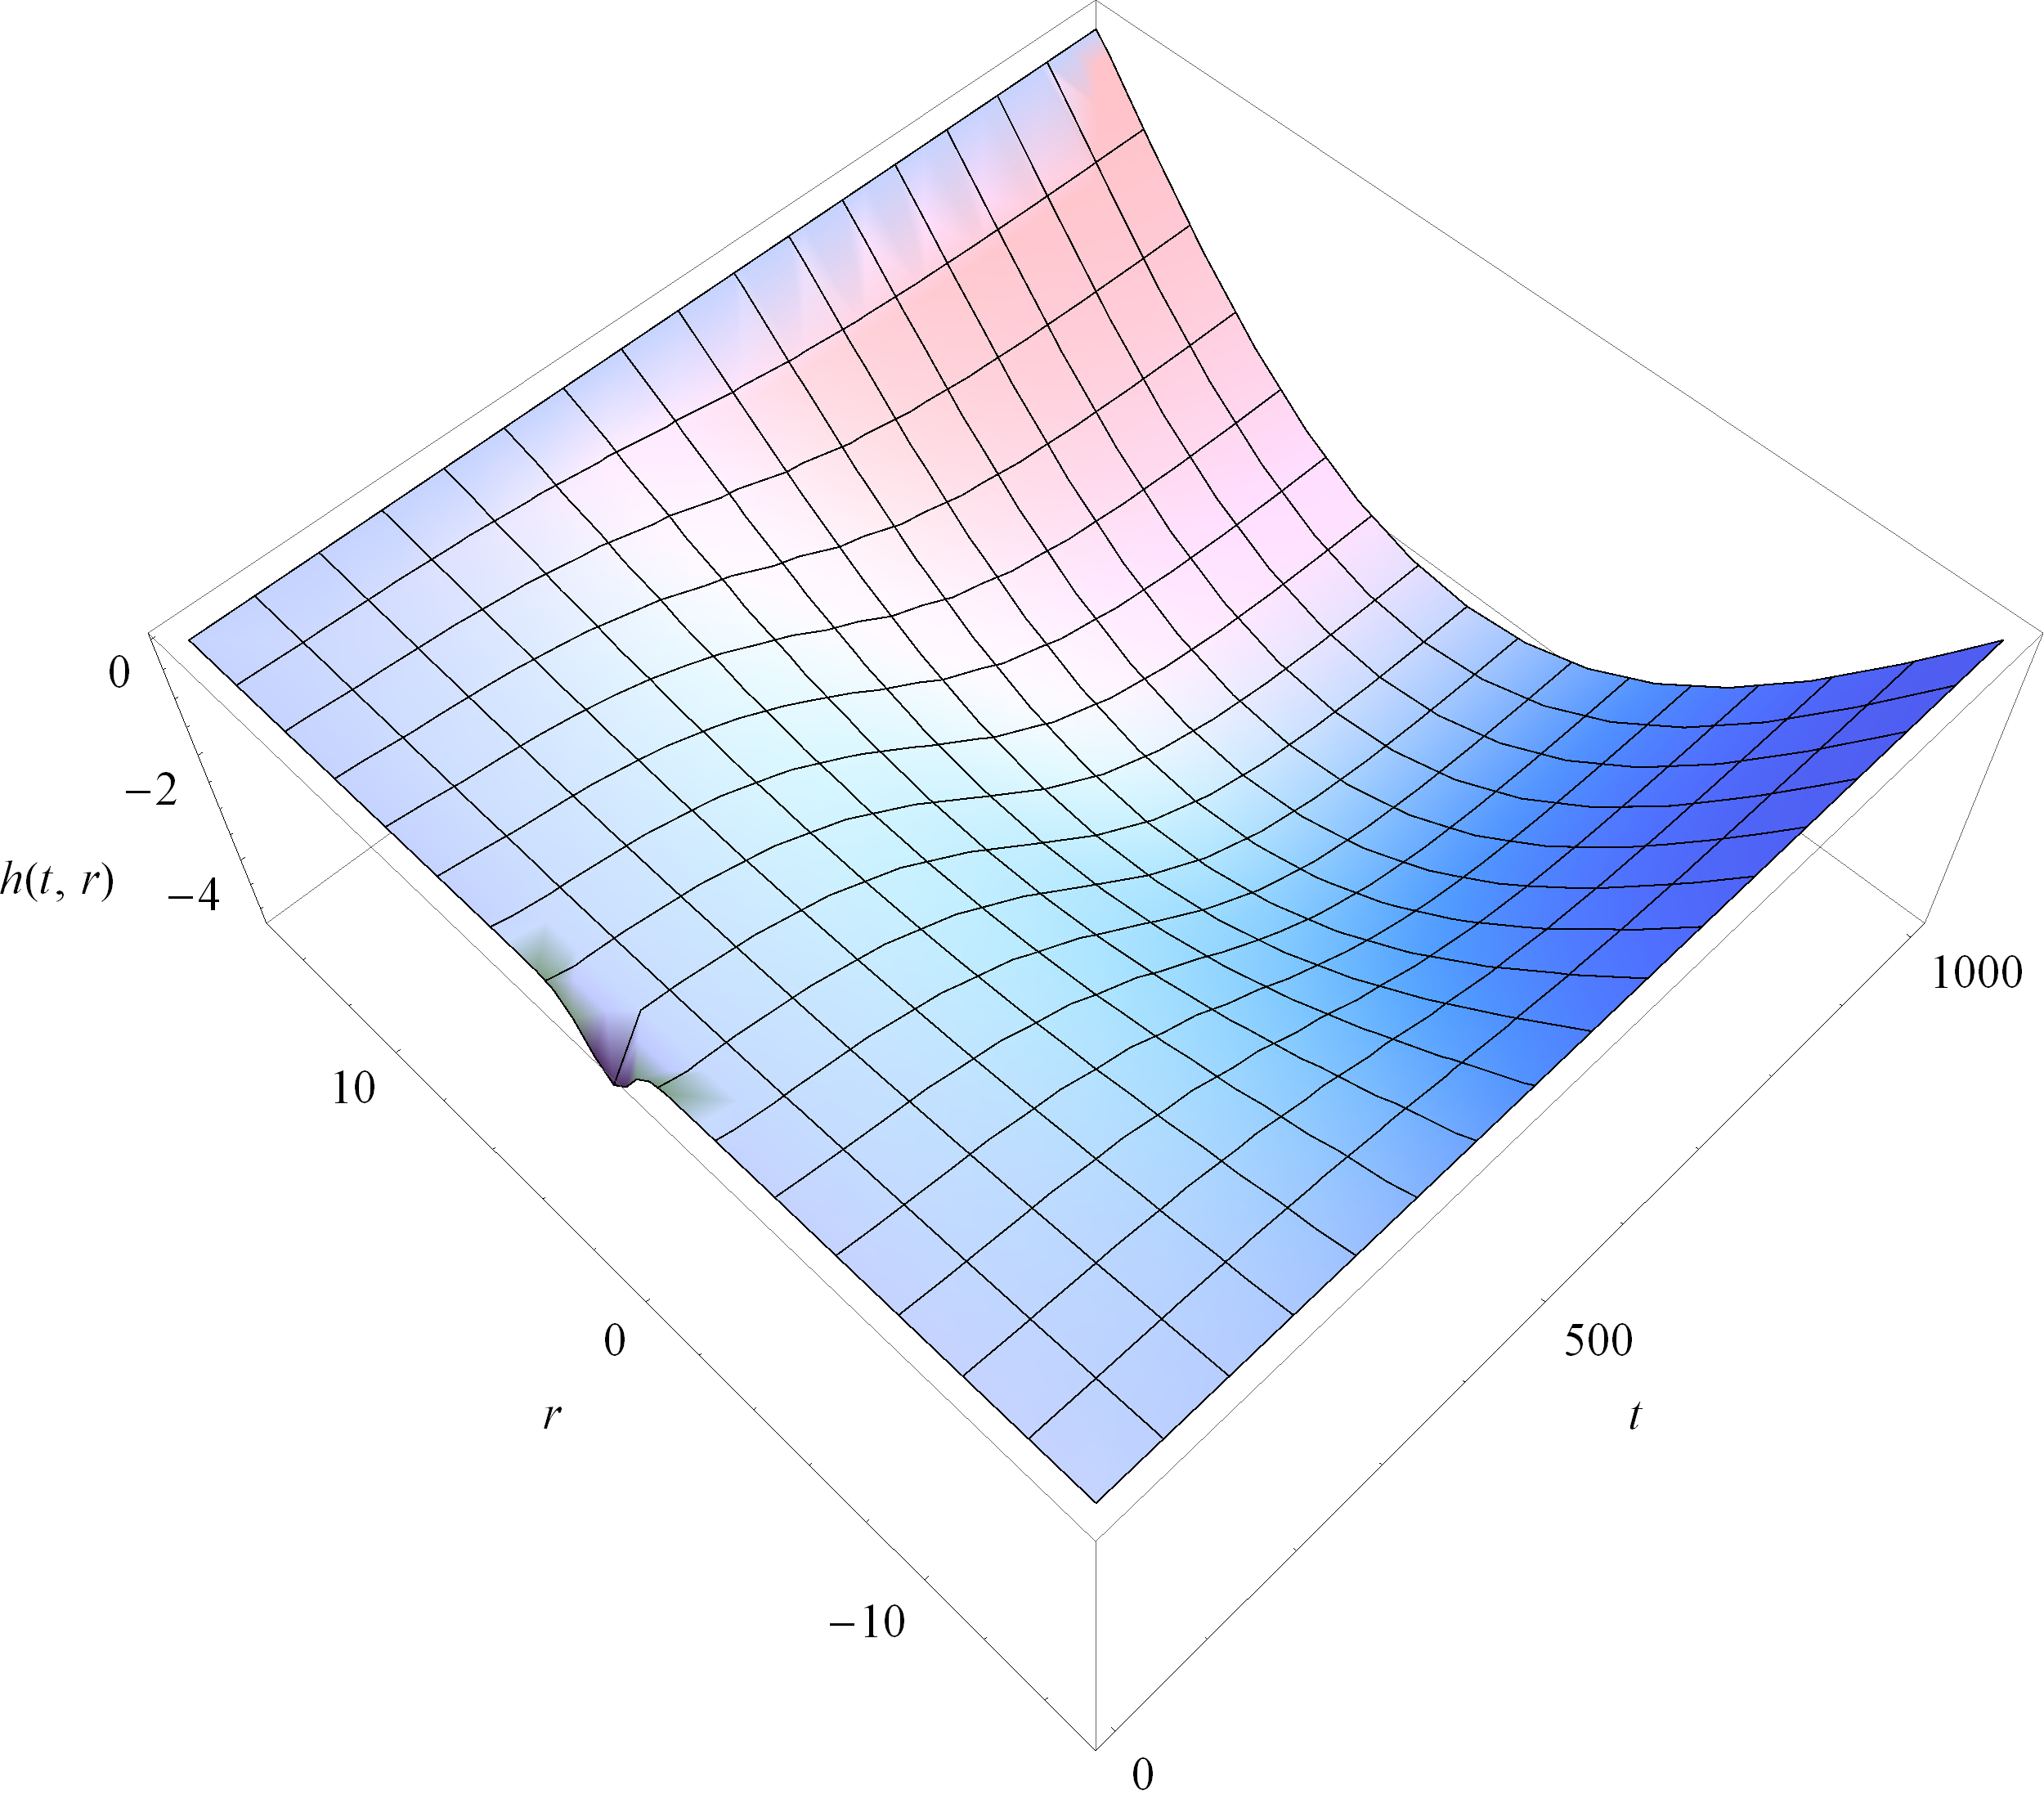
\includegraphics[width=9cm]{slike/difuzija-logisticna-rast2}
      \end{center}
      \caption{Vzeli smo $D=1$, $a=\frac{1}{50}$, $K=-10$.}
      \label{fig:difuzija-logisticna-rast}
    \end{figure}

    Vidimo, da ko se pobočje enkrat oblikuje, ne spreminja več oblike, ampak potuje kot valovna fronta navzven (Slika \ref{fig:difuzija-logisticna-rast}). Pokažemo lahko, da je dolžina vala odvisna od difuzijske konstante $D$ in faktorja rasti $a$, ter da velja: 

    \[ \lambda \sim \sqrt{D/a}. \]

    Iz te zveze lahko pokažemo tudi, da je hitrost takega vala $v = 2 \sqrt{D a}$.

    Enačba (\ref{difuzija-logisticna-rast}) se uporablja za opis zaželenih genov v populaciji, širjenje populacije v neposeljenem teritoriju, itn.
    Difuzivna logistična rast se zdi pri primerno izbranem faktorju $K$ zanimiv model za dinamiko vrtač.

    \subsection{Omejena eksponentna rast}

    Če izberemo $F(h) = a \cdot (K - h)$, dobimo:

    \begin{equation}
      \frac{ \partial h(t,x) }{ \partial t} = D \Delta h(t,x) + a \cdot (K - h(t,x)).
      \label{difuzija-omejena-eksponentna-rast}
    \end{equation}
    \begin{figure}[h]
      \begin{center}
        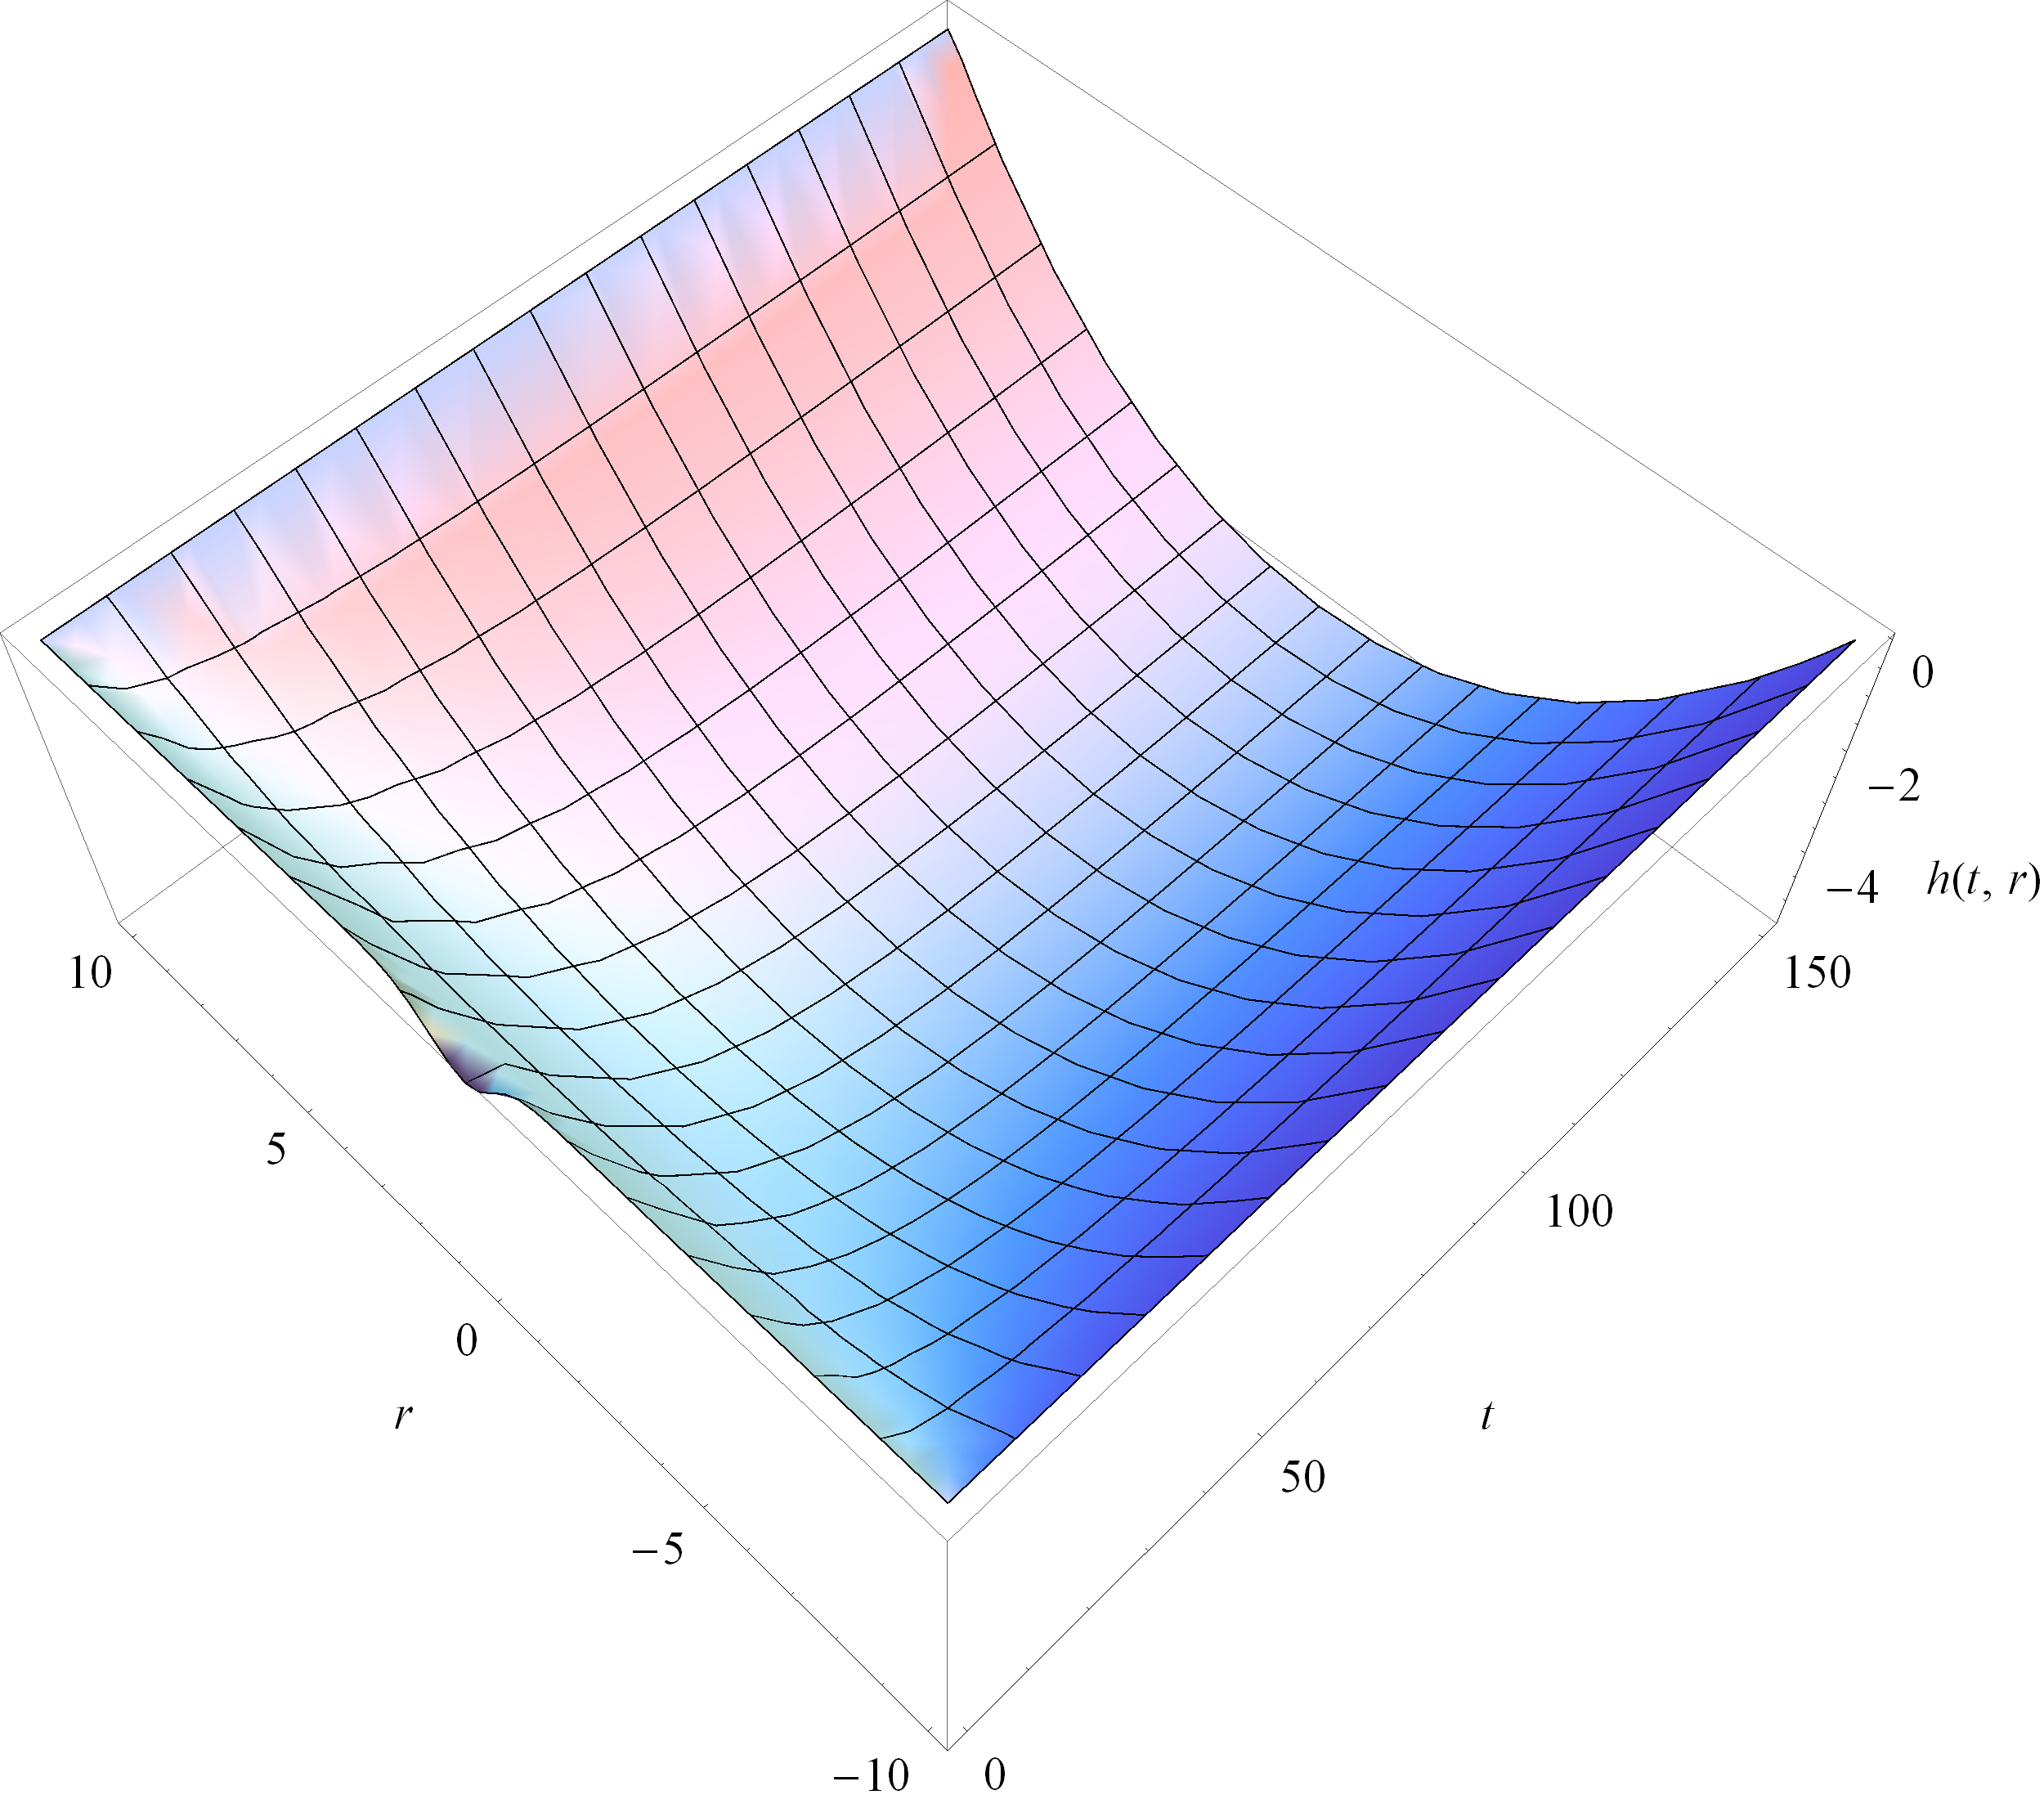
\includegraphics[width=9cm]{slike/difuzija-omejena-eksponentna-rast2}
      \end{center}
      \caption{Vzeli smo $D=1$, $a=\frac{1}{50}$, $K=-10$.}
      \label{fig:difuzija-omejena-eksponentna-rast}
    \end{figure}

    Tako dobljena rast (Slika \ref{fig:difuzija-omejena-eksponentna-rast}) eksponentno raste do praga K, kjer se zasiti. Rast v poljubni točki je neodvisna od stanja v sosednjih. Ta model se ne zdi najbolj verjeten kandidat za dinamiko vrtač.

    \subsection{Gompertzova rast}

    Če izberemo $F(h) = - h \cdot e^{-a t}$, dobimo:

    \begin{equation}
      \frac{ \partial h(t,x) }{ \partial t} = D \Delta h(t,x) - h(t,x) \cdot e^{-a t}.
      \label{difuzija-gompertzova-rast}
    \end{equation}
    \begin{figure}[h]
      \begin{center}
        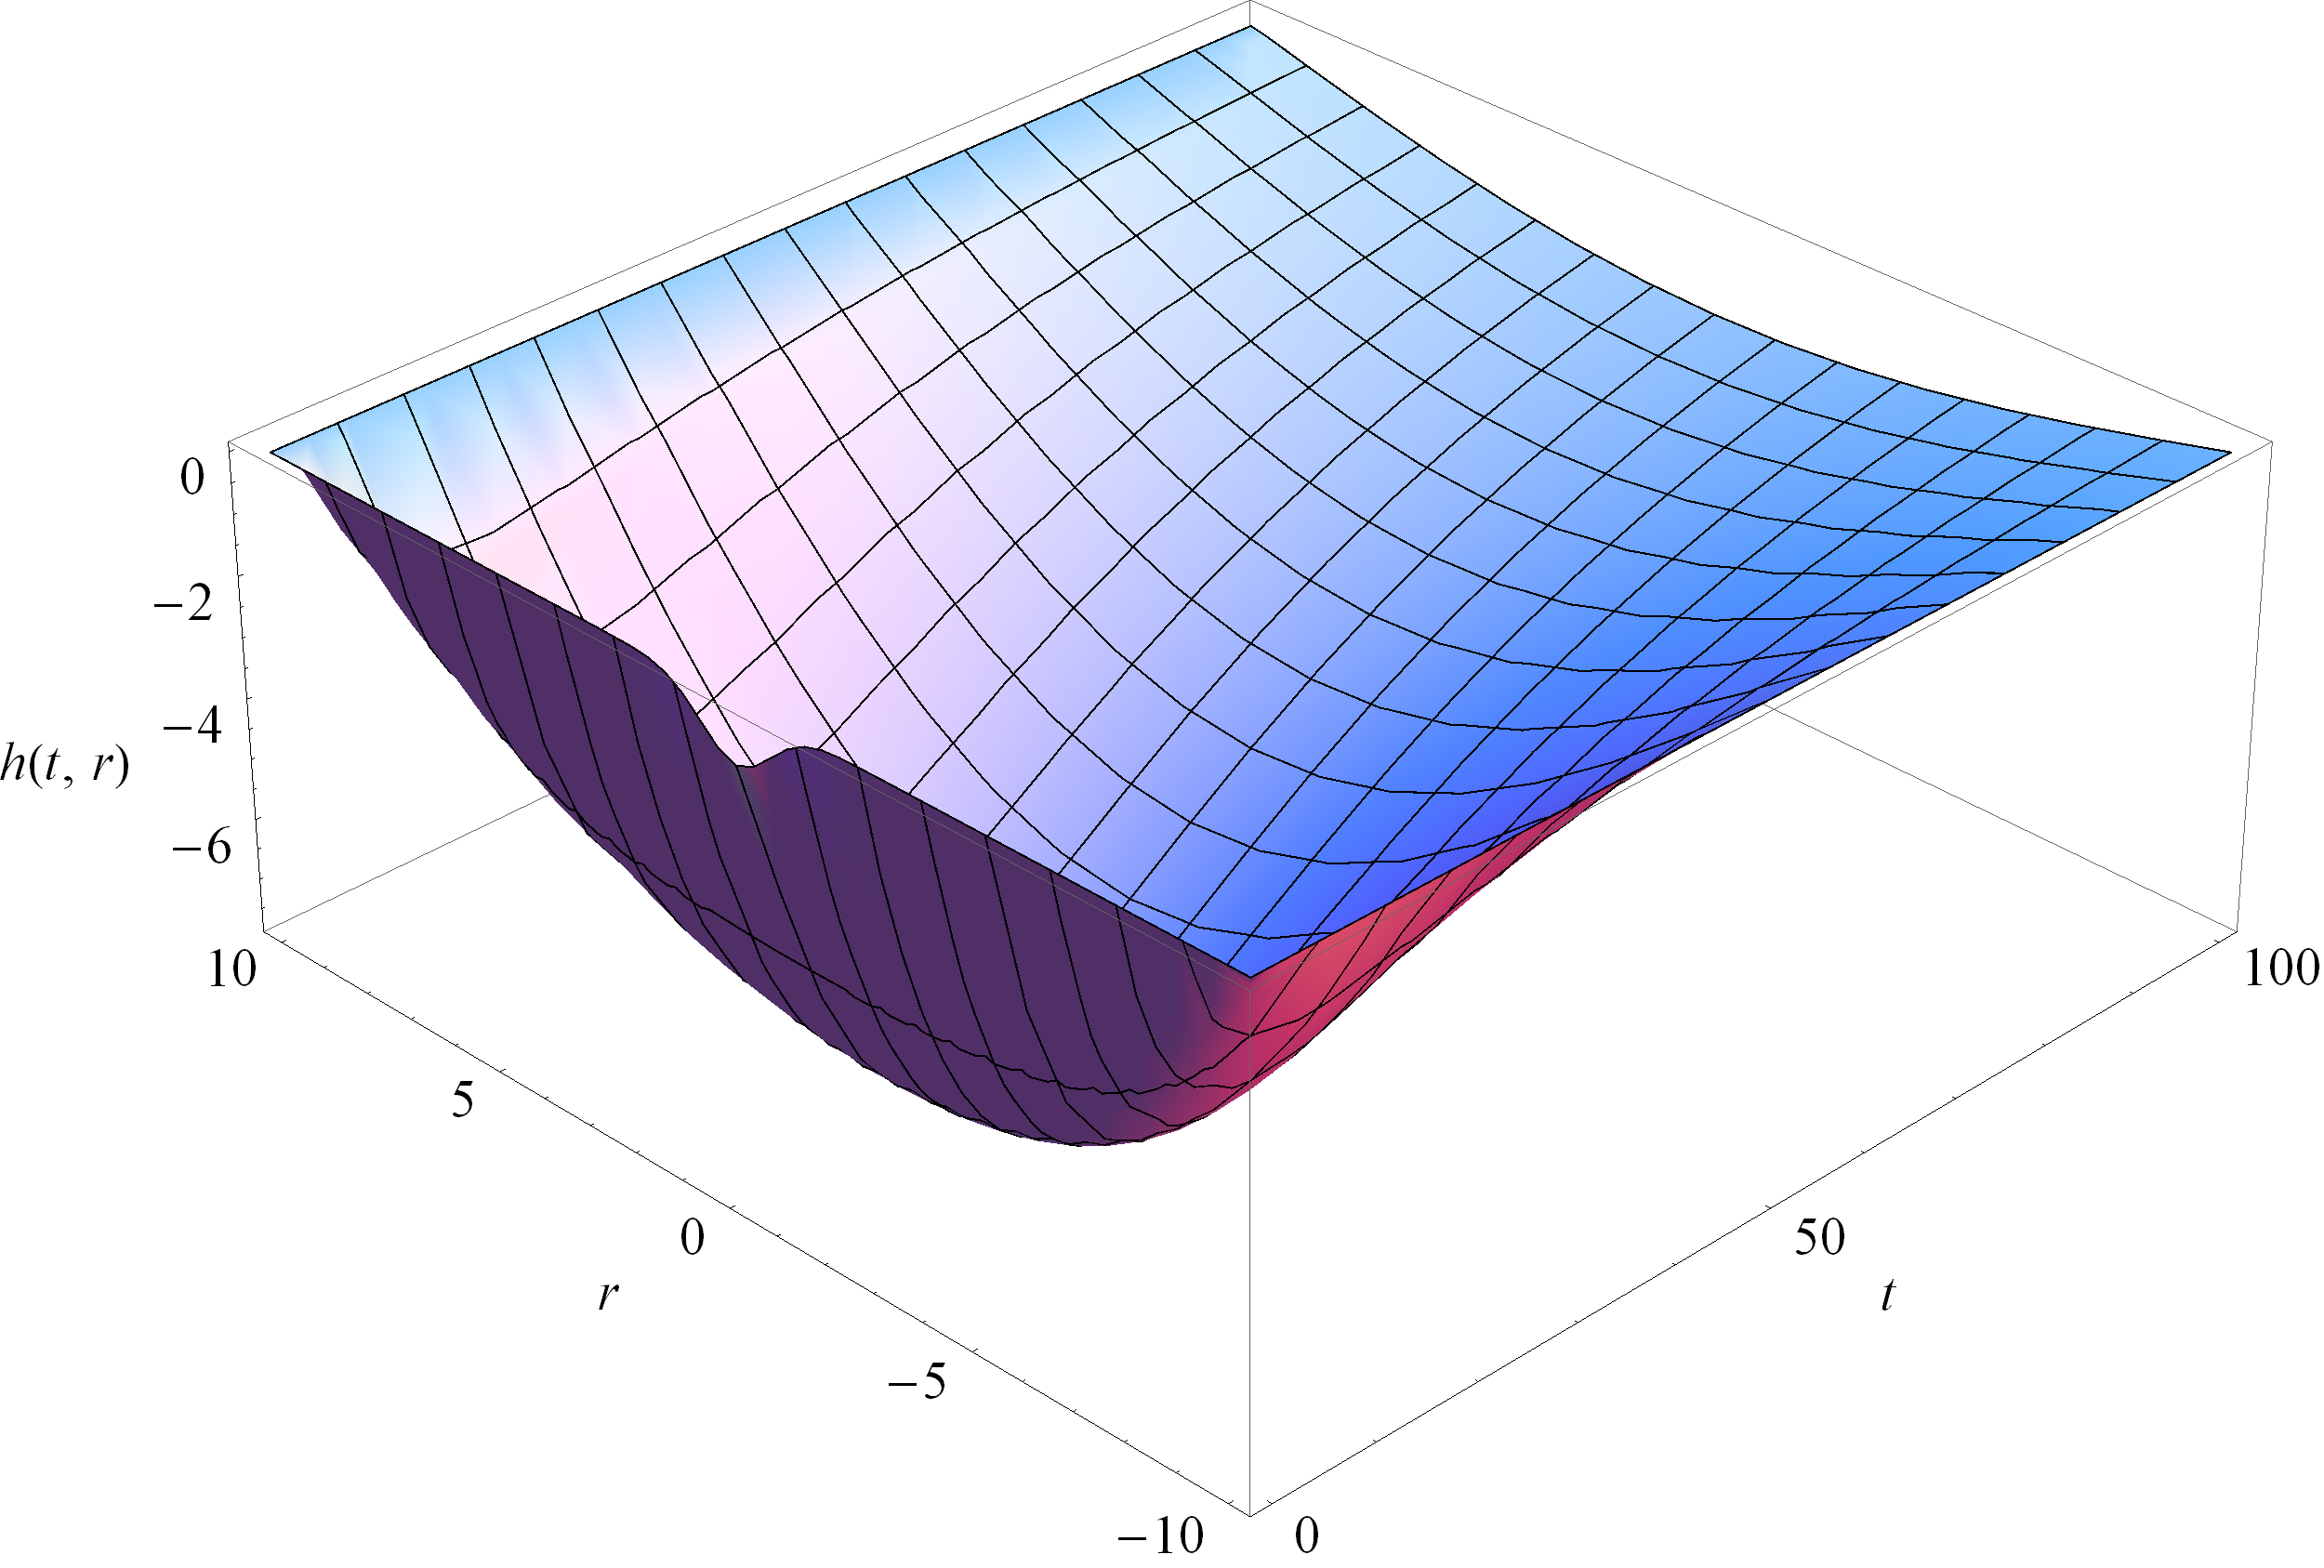
\includegraphics[width=9cm]{slike/difuzija-gompertzova-rast2}
      \end{center}
      \caption{Vzeli smo $D=1$, $a=\frac{1}{10}$.}
      \label{fig:difuzija-gompertzova-rast}
    \end{figure}

    Vidimo, da rast tokrat s časom upada (Slika \ref{fig:difuzija-gompertzova-rast}). Tako profil najprej zraste, nato pa se difuzijsko izravna, ko difuzija prevlada.
    Model se zdi za modeliranje vrtač neprimeren, saj nimamo jasne razlage, kaj bi povzročilo faktor rasti, ki bi nato eksponentno zamrl.
\newpage
[TODO]Primerjava vseh fenomenoloških reakcijsko difuzijskih modelov in njihove primernosti za opis našega problema.[TODO]

    \chapter{Zaključek}

    Izkaže se, da je zaznava in segmentacija vrtač na digitalnem modelu reliefa relativno enostavna naloga, izvedljiva na osebnem računalniku. Kodo, ki sem jo za ta postopek spisal, sem dokumentirano objavil na spletu in bo morda služila za obsežnejšo katalogizacijo vrtač.
    Za nekoliko težjo nalogo se izkaže določanje idealne oblike vrtače, saj le-ta ne obstaja. Pravo vprašanje bi se moralo glasiti, kakšna je idealna oblika vrtače na izotropni podlagi po dolgem času. Vseeno sem se odločil, da za idealno vrtačo vzamem povprečje velike količine vrtač.
    Precej zahtevnejša naloga je bila izbira fizikalnega modela in dinamičnega opisa vrtače zaradi omejene količine podatkov o časovni dinamiki (domnevali smo, da so vse vrtače že v ravnovesnem stanju) in nepoznavanja dejanskega procesa, ki znižuje površje.

    Kardar-Parisi-Zhangova rast površin nam da rezultat podoben kraškemu površju z vrtačami. Teoretično napovedan eksponent hrapavosti pa se relativno dobro ujema z izmerjenim na področju Menišije. Teh rezultatov ne moremo obravnavati kot dokaz, morda le spodbudo za nadaljnji študij.

    Za nepopoln model dinamike rasti vrtač predlagajmo model difuzijsko logistične rasti (\ref{fig:difuzija-logisticna-rast}), ki se zdi fizikalno najbolj smiseln.

    Za popolnejši študij in dober model vrtač bi verjetno potrebovali bolj poglobljene informacije o prsti, geoloških in bioloških dejavnikih, ki lahko vplivajo na časovno dinamiko terena. Zanimiva ideja bi bila z geološkim študijem najti in datirati vrtače v različnih stopnjah razvoja ter s pomočjo te informacije oblikovati dinamičen nastavek, na podlagi katerega bi potem morda bolj osvetlili dinamično enačbo. \newline
[TODO] \newline
- povzetek kaj ste naredili \newline
- povzetek glavnih rezultatov \newline
- kaj bi se še dalo oizboljšati \newline
[TODO]

\chapter{Priloge}

 \begin{figure}[H]
    \begin{center}
      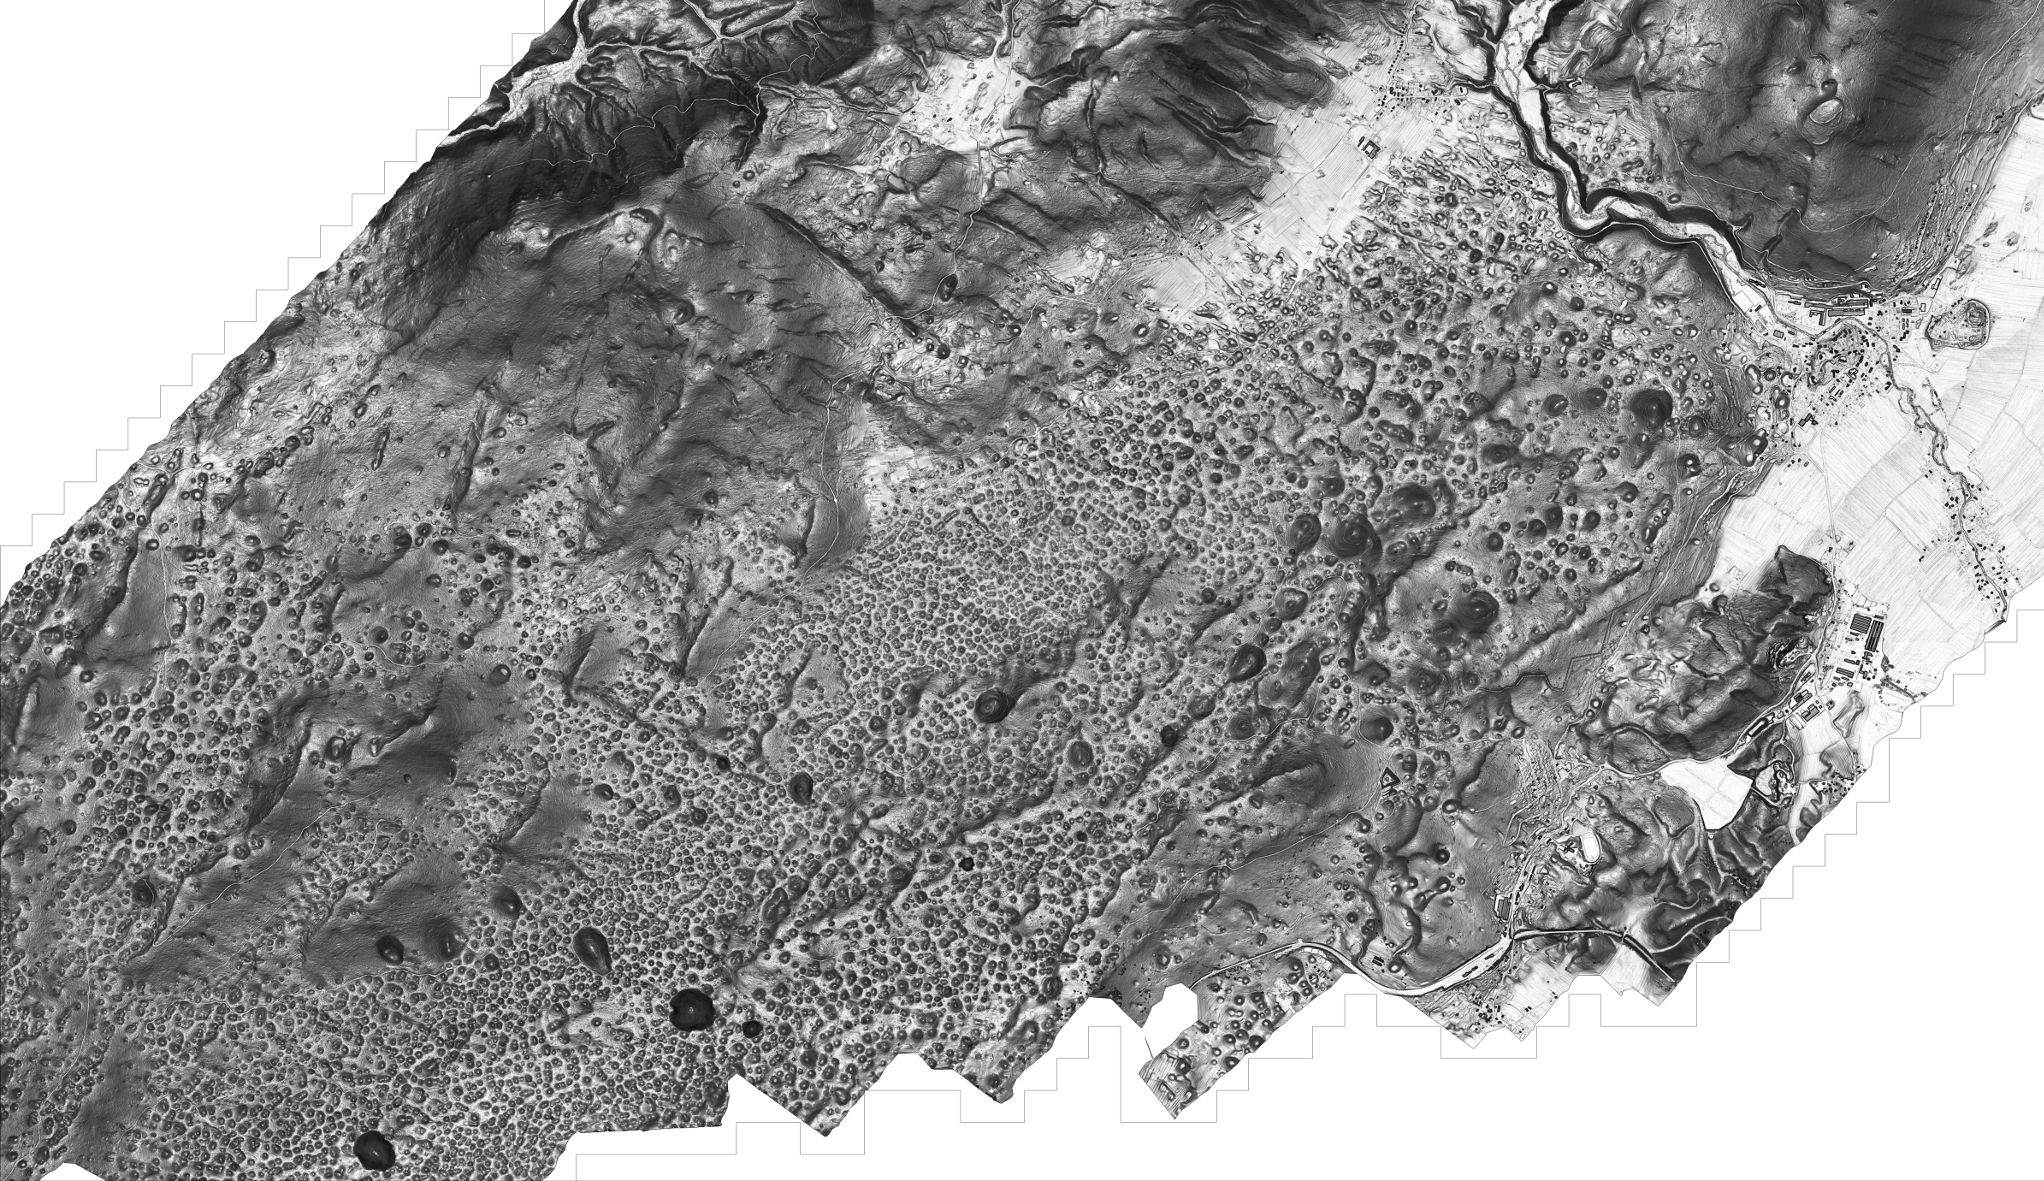
\includegraphics[width=10cm]{slike/menisija-relief}
    \end{center}
    \caption{Senčen digitalni model reliefa dela Menišije uporabljen v tej nalogi. Vir: Geodetski inštitut Slovenije \cite{LAK} po metodi \cite{Kobler20079}.}
    \label{fig:menisija-relief}
  \end{figure}


    \newpage \thispagestyle{empty}


    \nocite{*}
    \newpage
    \bibliography{bibliography}{}
    \addcontentsline{toc}{chapter}{Literatura}
    \bibliographystyle{alpha}

    \newpage \thispagestyle{empty}



    \vspace*{1cm}
    \begin{center} {\Large \textbf{\sc Izjava o avtorstvu in objavi elektronske oblike zaključnega dela: }} \end{center}

      \vspace{1cm} \noindent Podpisani Rok Mihevc izjavljam:
      \noindent 

      \begin{itemize}
        \item 
          da sem diplomsko delo z naslovom \emph{Kraške vrtače Dinarskega krasa} izdelal samostojno pod mentorstvom prof.\ dr.\ \mbox{Rudolfa} \mbox{Podgornika} in
        \item
          da Fakulteti za matematiko in fiziko Univerze v Ljubljani dovoljujem objavo elektronske 
          oblike svojega dela na spletnih straneh.
      \end{itemize}

      \vspace{1cm} \noindent Ljubljana, 18. april 2014 \hfill Podpis avtorja:


      \end{document}

